% report.tex
% main file for the project report.

\documentclass[a4paper,titlepage,12pt]{scrreprt}

% utf-8
\usepackage{polyglossia}
\setdefaultlanguage[babelshorthands]{ngerman}
\usepackage{fontspec}

% german names
\usepackage{ngerman}

% colored links
\usepackage{color}
\usepackage[colorlinks]{hyperref}
\definecolor{grey}{rgb}{0.2,0.2,0.2}
\definecolor{orange}{rgb}{1,0.3,0}
\definecolor{turqoise}{rgb}{0,0.7,0.5}

% code listings
\usepackage{listings}
\lstset{%
	basicstyle={\ttfamily \small},
	breaklines=true,
	commentstyle=\color{grey},
	keywordstyle=\color{orange},
	language=C,
	numbers=left,
	showspaces=false,
	stringstyle=\color{turqoise},
	xleftmargin=20pt
}

% graphics
\usepackage{graphicx}
\graphicspath{{images/}}

% fancy headers and footers
\usepackage{fancyhdr}
\pagestyle{fancy}
% clear style
\fancyhead{}
\fancyfoot{}
% new style
\renewcommand{\chaptermark}[1]{%
	\markboth{\thechapter.\ #1}{}
}
\renewcommand{\sectionmark}[1]{%
	\markright{\thesection.\ #1}{}
}
\renewcommand{\headrulewidth}{0.5pt}
\renewcommand{\footrulewidth}{0.5pt}
\fancyhead[LE,RO]{\rightmark}
\fancyhead[LO,RE]{\leftmark}
\fancyfoot[LE,RO]{\thepage}
\fancyfoot[LO,RE]{MMK Sommersemester 2015}
\fancypagestyle{plain}{%
	\fancyhf{}
	\renewcommand{\headrulewidth}{0pt}
	\renewcommand{\footrulewidth}{0.5pt}
	\fancyfoot[LE,RO]{\thepage}
	\fancyfoot[LO,RE]{MMK Sommersemester 2015}
}

% no indented paragraphs
\usepackage{parskip}

% TODO: what's this?
\setkomafont{disposition}{\normalfont\bfseries}

% for verbatiminput
\usepackage{verbatim}

% not yet used
%\input{src/cmd}

\begin{document}

\titlehead{
	
\includegraphics[width=0.9\linewidth]{hska_logo}
}

\title{Dokumentation: \\ Pro-Kontra Liste}
\subtitle{Mensch-Maschine Kommunikation}
\author{%
	Tobias Kerst, 47646 \\
	Maike Rees, 47307 \\
	Patrick König, 46910
}
\date{Sommersemester 2015}
\publishers{
    \textbf{Dozent:} Prof. Dr. rer. nat. Bröckl
}
\maketitle

\clearpage

\begingroup
\hypersetup{linkcolor=black}
\tableofcontents
\endgroup

\clearpage

\chapter{Themenstellung}
\label{chap:intro}

In der vorliegenden Hausarbeit widmen wir uns der Dokumentation zu einer Anwendung für Professoren und Studenten. Diese dient dazu, während der Vorlesung Pro- und Kontra-Argumente zu einem vom Professor vorgegebenem Thema zu sammeln. 
Für Studenten wird die Anwendung in Form einer Android-Application (kurz AA) verfügbar sein. Der Professor verwendet eine mit dem Beamer kompatible Webanwendung. In dieser WebApp kann er  das Thema erstellen und die von den Studenten eingeschickten Argumente verwalten, sortieren und ordnen.
Hierbei spielen interaktive Bedienelemente zur Verwaltung der gesammelten Informationen eine zentrale Hauptrolle. 

Die Anforderungen an die App sind je nach Nutzer unterschiedlich. Der Studenten soll durch einfach verständliche Funktionen in seinem Bestreben, sich in der Vorlesung einzubringen unterstützt werden. Für ihn ist das abgeben von Argumenten die zentrale Funktion. Diese soll durch möglichst wenig Klicks erreicht werden. Der Student kann die bereits abgegebenen Argumente seiner Kommilitonen einsehen und eventuell bewerten. 
Für den Professor ist das Erstellen einer Thematik und die Auswertung, Sortierung und Besprechung aller eingeschickten Argumente die zentrale Aufgabe, bei der die App ihn unterstützen muss. Hierbei soll auch eine Regelsystem berücksichtigt werden, damit  die Studenten die Funktionen der App nicht missbrauchen können. Der Professor muss die Argumente nach Relevanz, Redundanz, Zusammengehörigkeit etc. sortieren können. Auch das Löschen einzelner Argumente soll berücksichtigt werden (z.B. bei Dopplung). Der Professor kann die Umfragen als PDF exportieren. Er kann diese PDF an alle mitwirkenden Studenten und interessierte Kollegen verschicken. 

Von technischer Seite her sollen die Themen vom Rechner / Laptop des Professors auf die Smartphones der Studenten über Bluetooth übertragen werden. Es soll einen Offline-Modus geben, mit der die Themen auch ohne Bluetooth-Verbindung von zu Hause ergänzt werden können. 
Jedes Thema bekommt vom Professor einen begrenzten Zeitraum zugewiesen. Nur in diesem Zeitraum können die Studenten Argumente zum Thema beitragen. Danach gilt das Thema als geschlossen.

Die nächste Teilaufgaben stellen sich wie folgt dar:
\begin{itemize}
\item Klärung aller Funktionen
\item Erstellen mehrere Storyboards (pro Person eines)
\item Festlegen auf ein gemeinsames Storyboard
\item Chancen und Risiken zusammentragen
\item Personas erstellen
\item Objekt-Hierarchie und Bedienelemente festlegen
\end{itemize}






\chapter{Analyse}
\label{chap:analyse}

\section{Chancen und Risiken}
\label{sec:chances}

Chancen und Risiken
Die App soll die Studenten besser in die Vorlesung mit einbeziehen. Sie soll aktivierend wirken und die Kreativität der Studenten anregen. Durch die Nutzung des Smartphones kommen auch introvertierte, unsichere und ängstliche nn zu Wort. Durch die Interaktion und die Auflockerung der Vorlesung sollen unmotivierte, tagträumende Studenten dazu animiert werden, sich einzubringen. 
Der Professor bekommt die Chance, die Denkweise der Studenten besser zu verstehen und kann sehen, wo noch Verständnis-Probleme vorhanden sind. Oftmals passiert es, dass eine abgehobene Denkweise entsteht, wenn man sich auf einem Gebiet spezialisiert. Es wird schwieriger Anfänger-Probleme und Fragen nachzuvollziehen oder überhaupt Problemquellen zu entdecken. Hierbei kann die App ebenfalls helfen. Die Vorlesung wird durch die Anwendung der  App interaktiver und somit höchstwahrscheinlich auch beliebter unter den Studenten.

Als Risiko sehen wir einen möglichen Missbrauch der App-Funktionen von Seiten der Studenten. Durch unqualifizierte, nicht zum Thema passende Beiträge kann die Vorlesung massiv gestört werden. 
Des Weiteren darf das Interface nicht zu komplex aufgebaut sein, um auch nicht-technik-affinen Benutzern einen einfachen Umgang mit der App zu gewähren. 
Es muss festgelegt werden, wie mit Unklarheiten in der Fragestellung des Professors umgegangen wird. Ein weiteres Risiko stellt die Bewertung der Studenten dar. Hierbei muss entschieden werden, ob die Argumente anonym abgegeben werden oder ob gezeigt wird, welcher Studenten das Argument verschickt hat, um auch eventuelle Rückfragen stellen zu können. Je nach Thema ist die Anonymisierung empfehlenswert, damit die Studenten sich eifriger einbringen und weniger Angst haben, über ihre Argumente zur Rede gestellt zu werden.

Auf technischer Seite gibt es ebenfalls Risiken. Zum einen muss die Art der Benutzerverwaltung geklärt werden. Es besteht die Möglichkeit, dass sich die Nutzer für die App einen eigenen Account anlegen müssen oder aber sich mit ihrer Hochschul- / Universitäts-E-Mail-Adresse einloggen. 
Des Weiteren ist die Verbindung zwischen den unterschiedlichen Geräten eine Schwierigkeit. Um gutes Arbeiten zu ermöglichen, muss die Verbindung permanent bestehen oder eine lokale Kopie auf dem Endgerät des Nutzers zur Verfügung stehen. Ebenfalls müssen die Nutzern passende Endgeräte besitzen.

\section{Personas}
\label{sec:personas}

\subsection{Torben Bruhns}

\begin{wrapfigure}{L}{0.35\textwidth}
  \vspace{-20pt}
  \begin{center}
    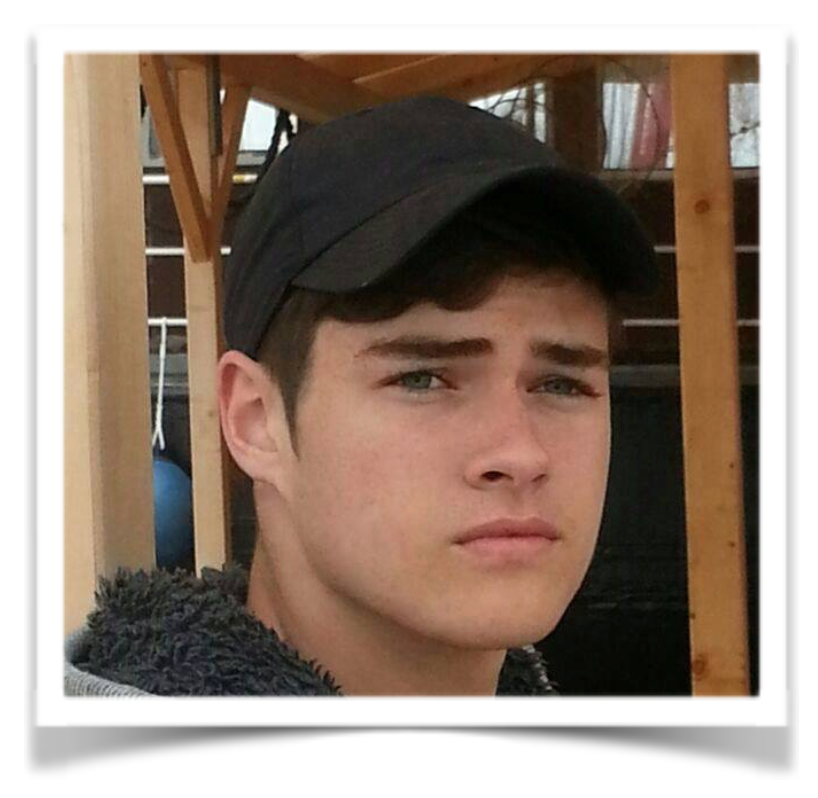
\includegraphics[width=0.32\textwidth]{./images/Torben_Bruhns}
  \end{center}
  \vspace{-40pt}
\end{wrapfigure}

\textbf{Name:} Torben Bruhns

\textbf{Alter:} 27

\textbf{Studium:} Informatik, 6. Semester

\textbf{Computerkenntnisse:} Sehr gut

\textbf{Ziele:} Bachelor- Abschluss schaffen durch so wenig Aufwand wie möglich 

\textbf{Vorlieben:} Computerspiele, Soziale Netzwerke, Aktive Benutzung komplizierter IDEs, Serien

\textbf{Motivation:} Interessiert sich für \texttt{ArguMens}, um den Dozenten fälschlicherweise von nicht existierendem Engangement zu überzeugen (Vortäuschen von aktiver Beteiligung).






\section{Fallstudien}
\label{sec:fallstudien}

\subsection{Herr Meier}

\paragraph{Ziel:} Herr Meier, Professor für Betriebssysteme, möchte mit seinen Studenten in der Vorlesung Vor- und Nachteile für bzw. gegen UNIX-Systeme sammeln. Sein Ziel dabei ist es, die Vorlesung etwas aufzulockern und nebenbei eine Lernerfolgskontrolle durchzuführen. 

\paragraph{Aktivitäten:}
\begin{itemize} 
\item öffnen der WebApp auf dem Laptop
\item mit Benutzername und Passwort einloggen
\item Eine neue Umfrage anlegen
\item Name der Umfrage, Vorlesung, Beschreibung, Zeitraum eintragen
\item Umfrage Speichern 
\item Umfrage überprüfen
\item Umfrage veröffentlichen
\item Ein Argument hinzufügen
\item Argumente verwalten
\end{itemize}


\subsection{Herr Tobias König}

\paragraph{Ziel:} Tobias König sitzt in der Vorlesung und möchte sich an der Pro- \and Contra-Argument Liste seines Professors beteiligen um sich bei diesem einzuschleimen.

\paragraph{Aktivitäten:}
\begin{itemize}
\item anschalten seines Smartphones
\item downloaden der ArguMens-App 
\item Einloggen mit Benutzername und Passwort
\item Auswählen der Umfrage
\item Eingeben eines Pro-Arguments
\item Eingeben eines weiteren Pro-Arguments
\item Eingeben eines Contra-Arguments
\item eine bereits beendete Umfrage anschauen
\item zurück zur aktuellen Umfrage springen
\item ein weiteres Contra-Argument ansehen
\end{itemize}

\subsection{Herr Patrick Kerst}

\paragraph{Ziel:} Patrick Kerst sitzt verärgert in der Vorlesung. Um seinen Frust abzulassen, möchte er Kritik in Argumente verpacken und auf die Pro-Contra-Liste setzen

\paragraph{Aktivitäten}
\begin{itemize}
\item öffnen der App
\item auswählen der gewünschten Umfrage
\item Eingeben eines Contra Arguments 
\item Eingeben eines weiteren Contra Arguments 
\item Eingeben eines weiteren Contra Arguments
\item schließen der App 
\end{itemize}

\clearpage

\chapter{Entwurf}
\label{chap:entwurf}


\section{Maike Rees}
\label{sec:rees}

\begin{wrapfigure}{L}{0.4\textwidth}
  \vspace{-20pt}
  \begin{center}
    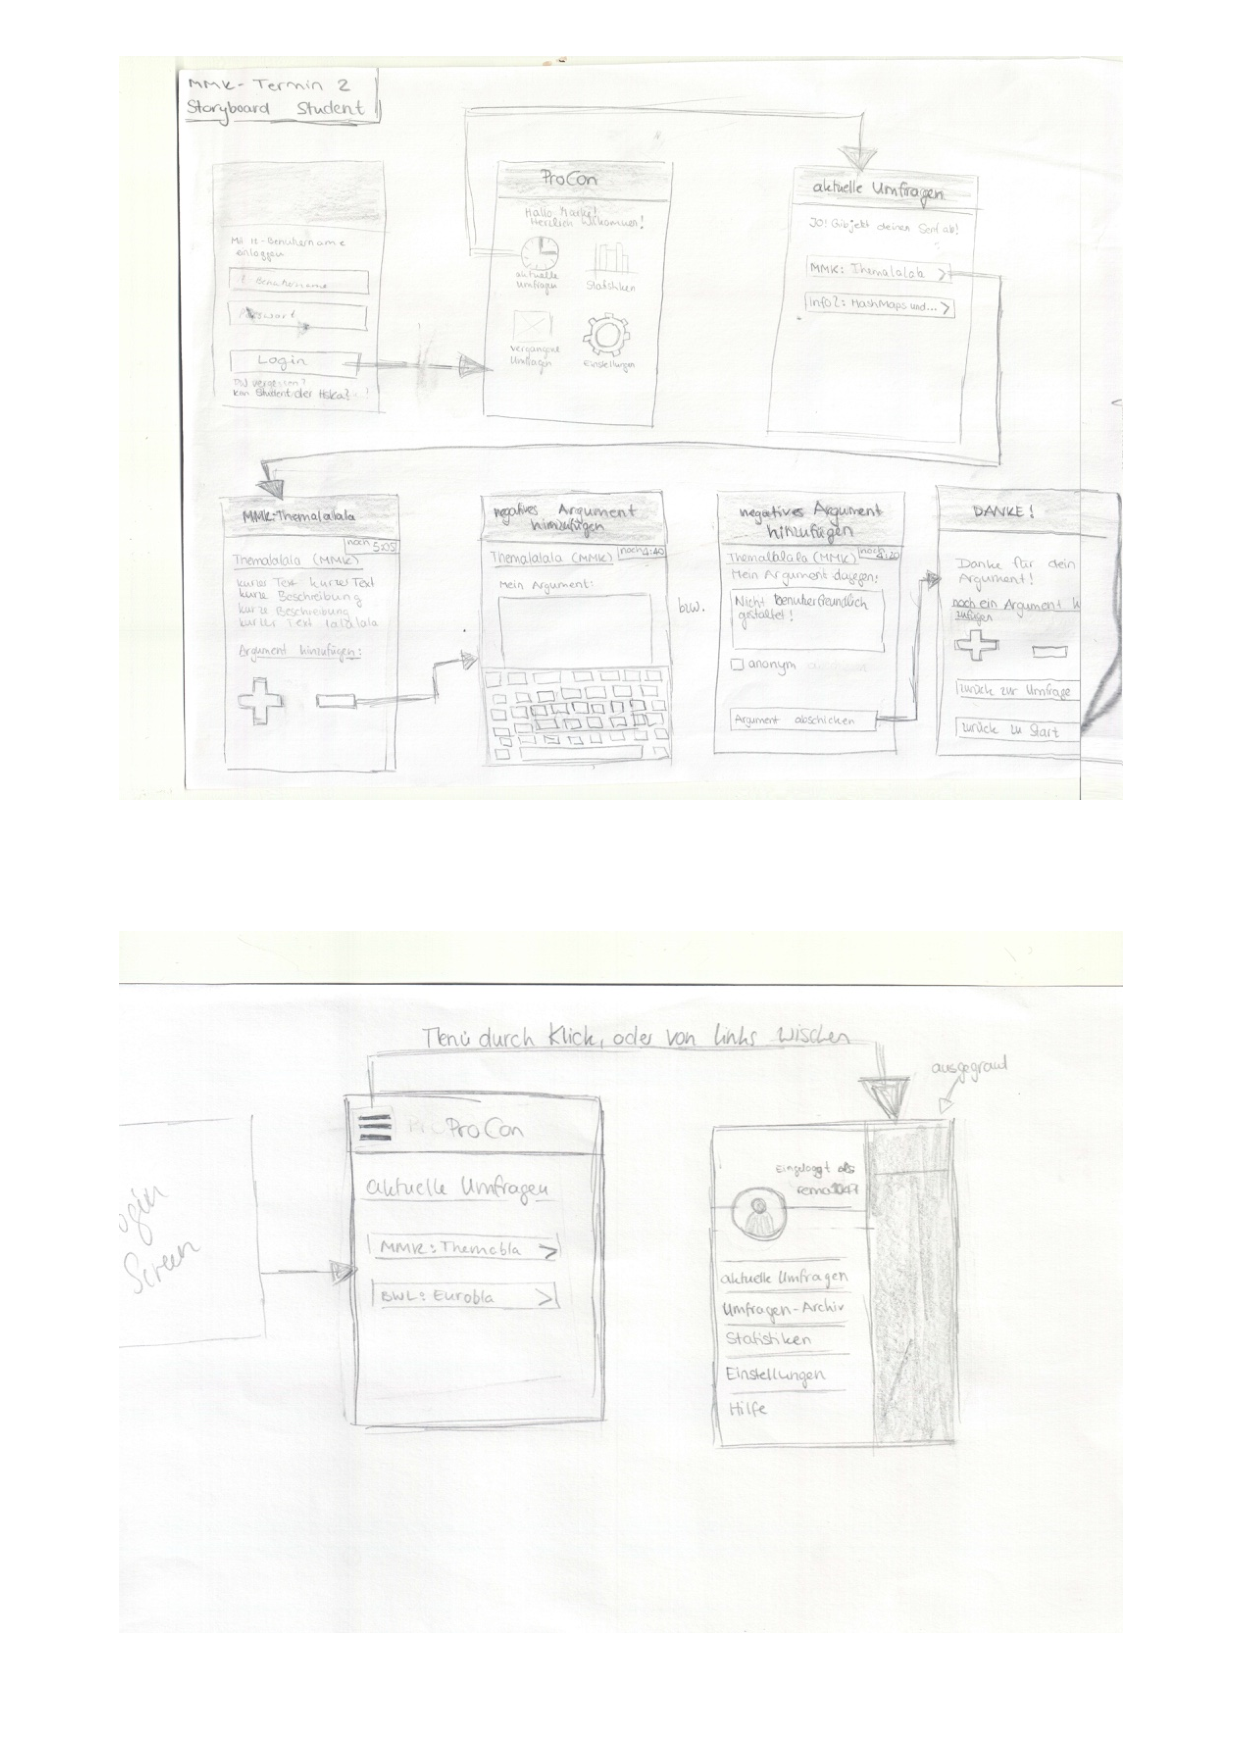
\includegraphics[page=1,width=0.85\textwidth]{./images/entwuerfe/maike}
  \end{center}
  \vspace{-40pt}
\end{wrapfigure}



\begin{wrapfigure}{L}{0.4\textwidth}
  \vspace{-20pt}
  \begin{center}
    \includegraphics[page=2,width=0.99\textwidth]{./images/entwuerfe/maike}
  \end{center}
  \vspace{-40pt}
\end{wrapfigure}



\begin{wrapfigure}{L}{0.4\textwidth}
  \vspace{-20pt}
  \begin{center}
    \includegraphics[page=3,width=0.99\textwidth]{./images/entwuerfe/maike}
  \end{center}
  \vspace{-40pt}
\end{wrapfigure}



\begin{wrapfigure}{L}{0.4\textwidth}
  \vspace{-20pt}
  \begin{center}
    \includegraphics[page=4,width=0.99\textwidth]{./images/entwuerfe/maike}
  \end{center}
  \vspace{-40pt}
\end{wrapfigure}

\clearpage



\section{Patrick König}
\label{sec:king}



\clearpage

\section{Tobias Kerst}
\label{sec:toby}

\begin{wrapfigure}{L}{0.4\textwidth}
  \vspace{-20pt}
  \begin{center}
    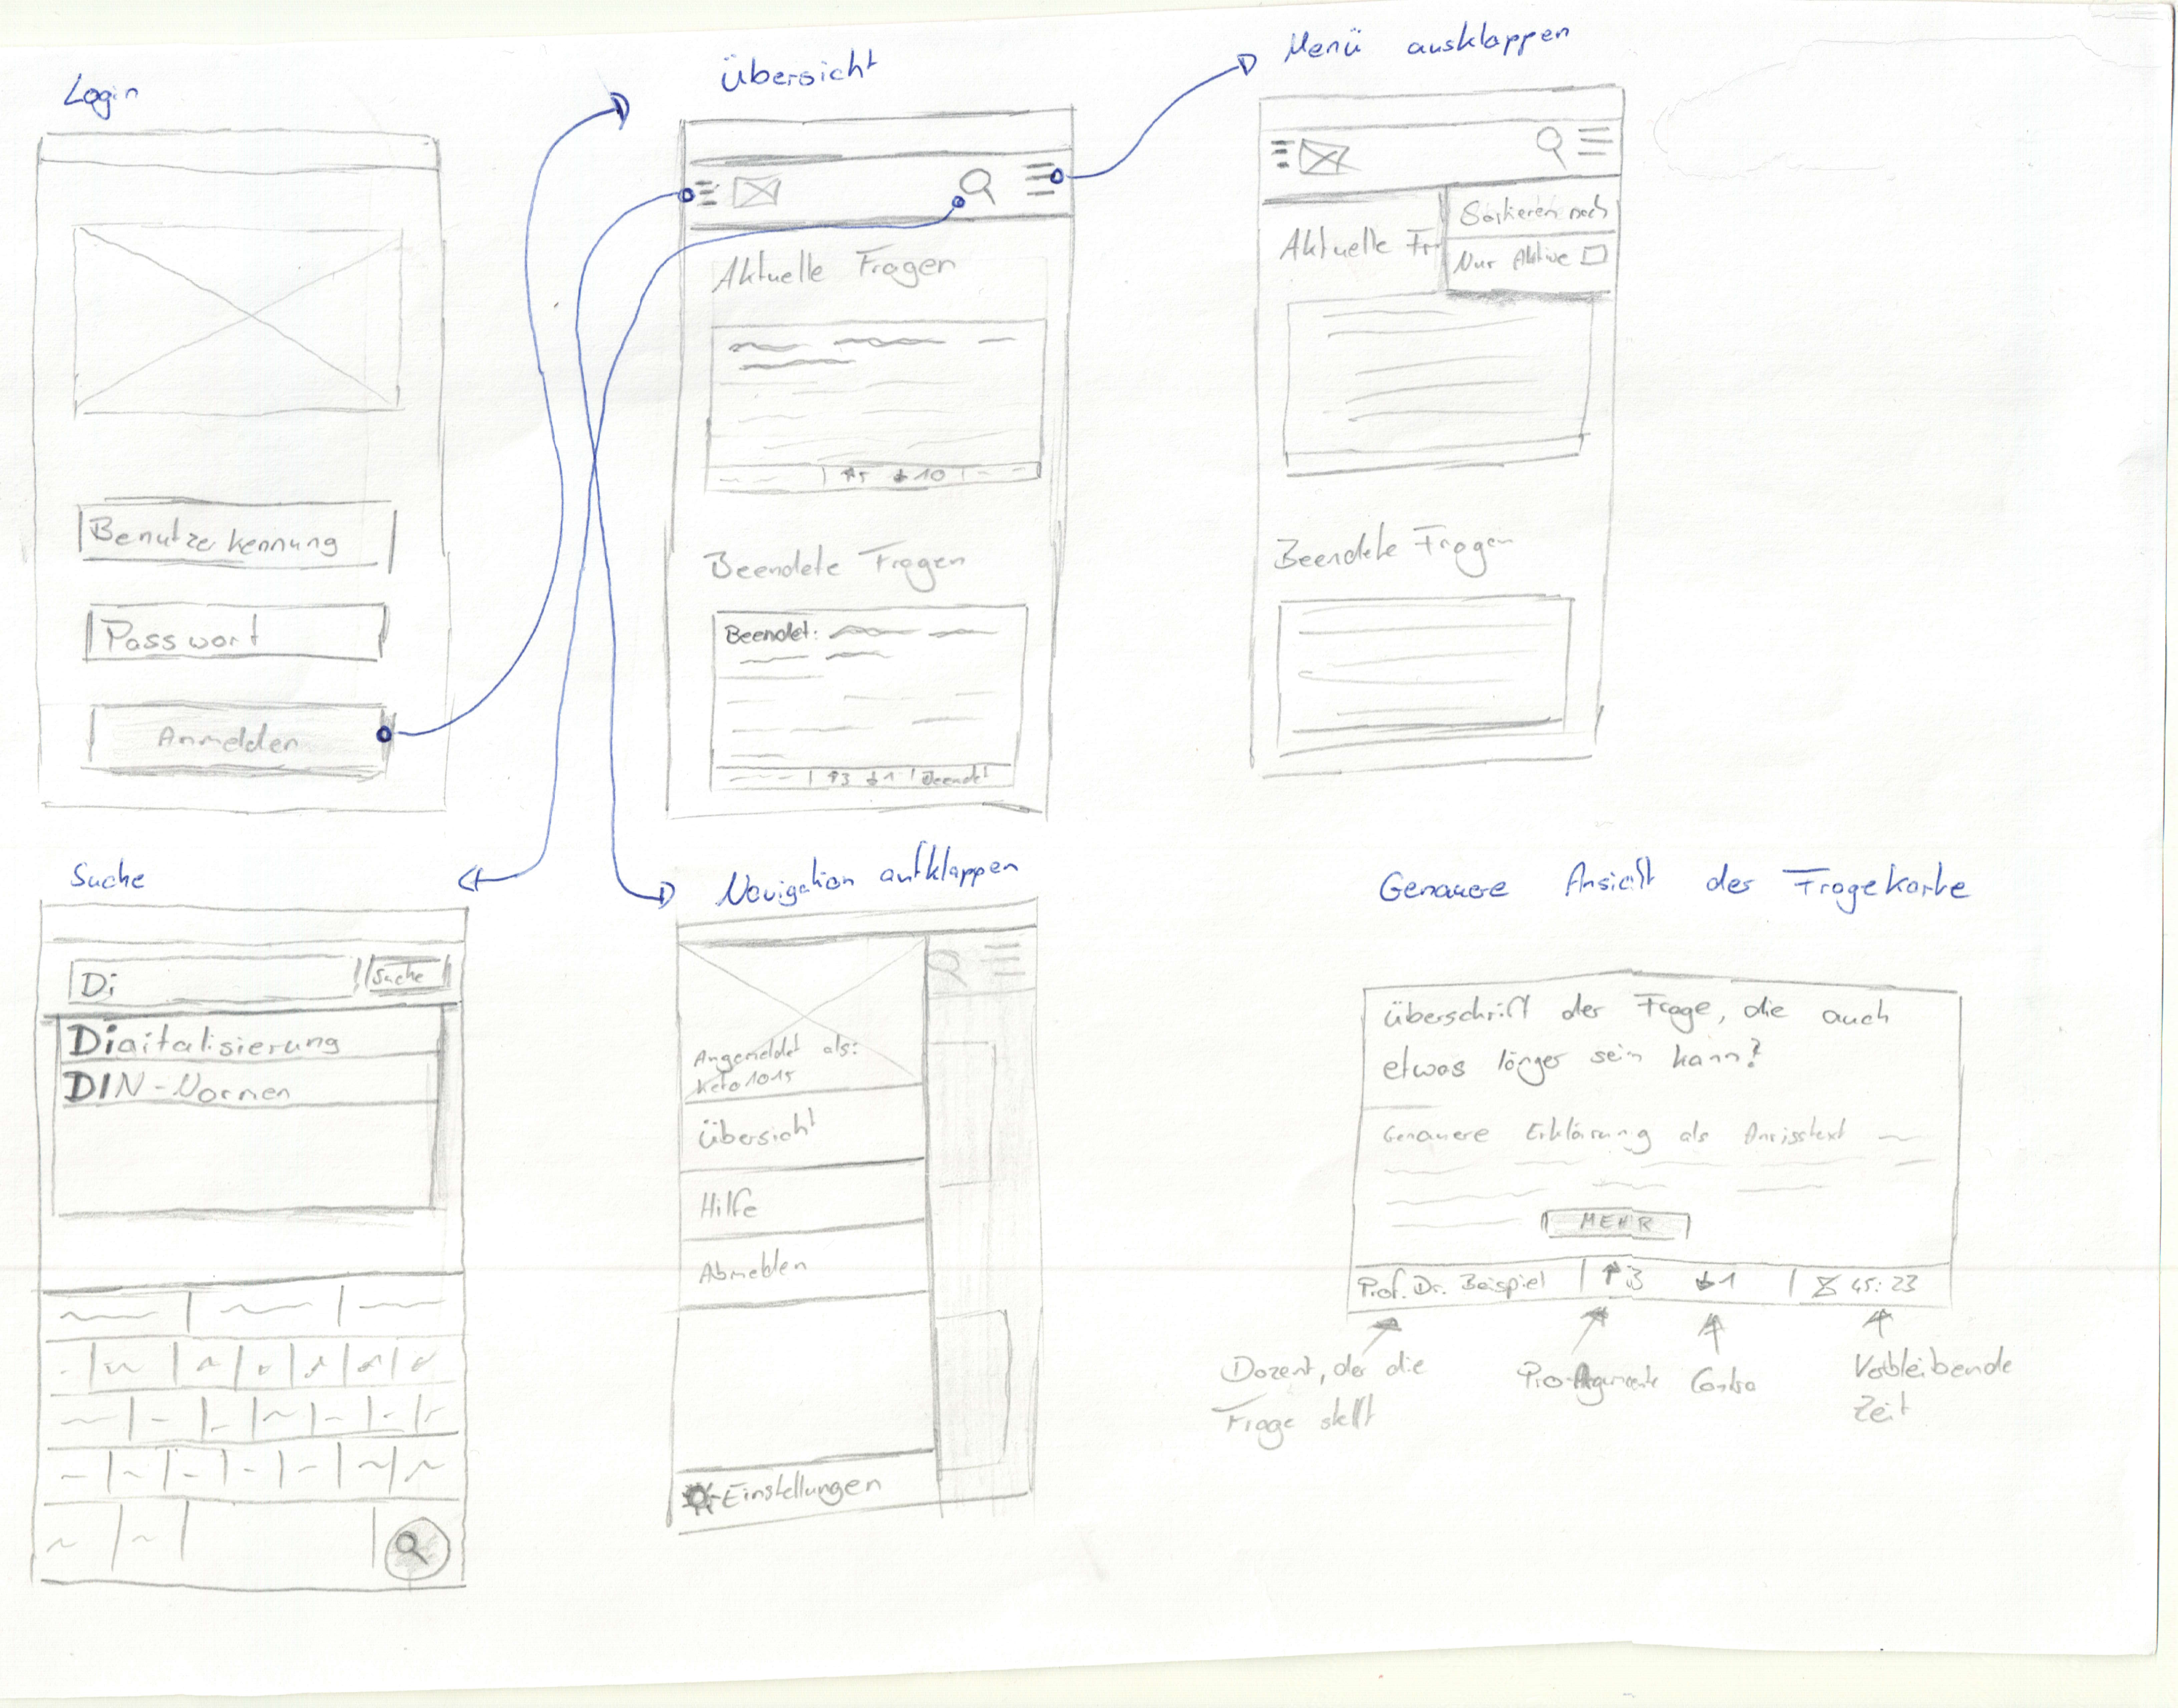
\includegraphics[width=0.99\textwidth]{./images/entwuerfe/toby1}
  \end{center}
  \vspace{-40pt}
\end{wrapfigure}

\clearpage
\begin{wrapfigure}{L}{0.4\textwidth}
  \vspace{-20pt}
  \begin{center}
    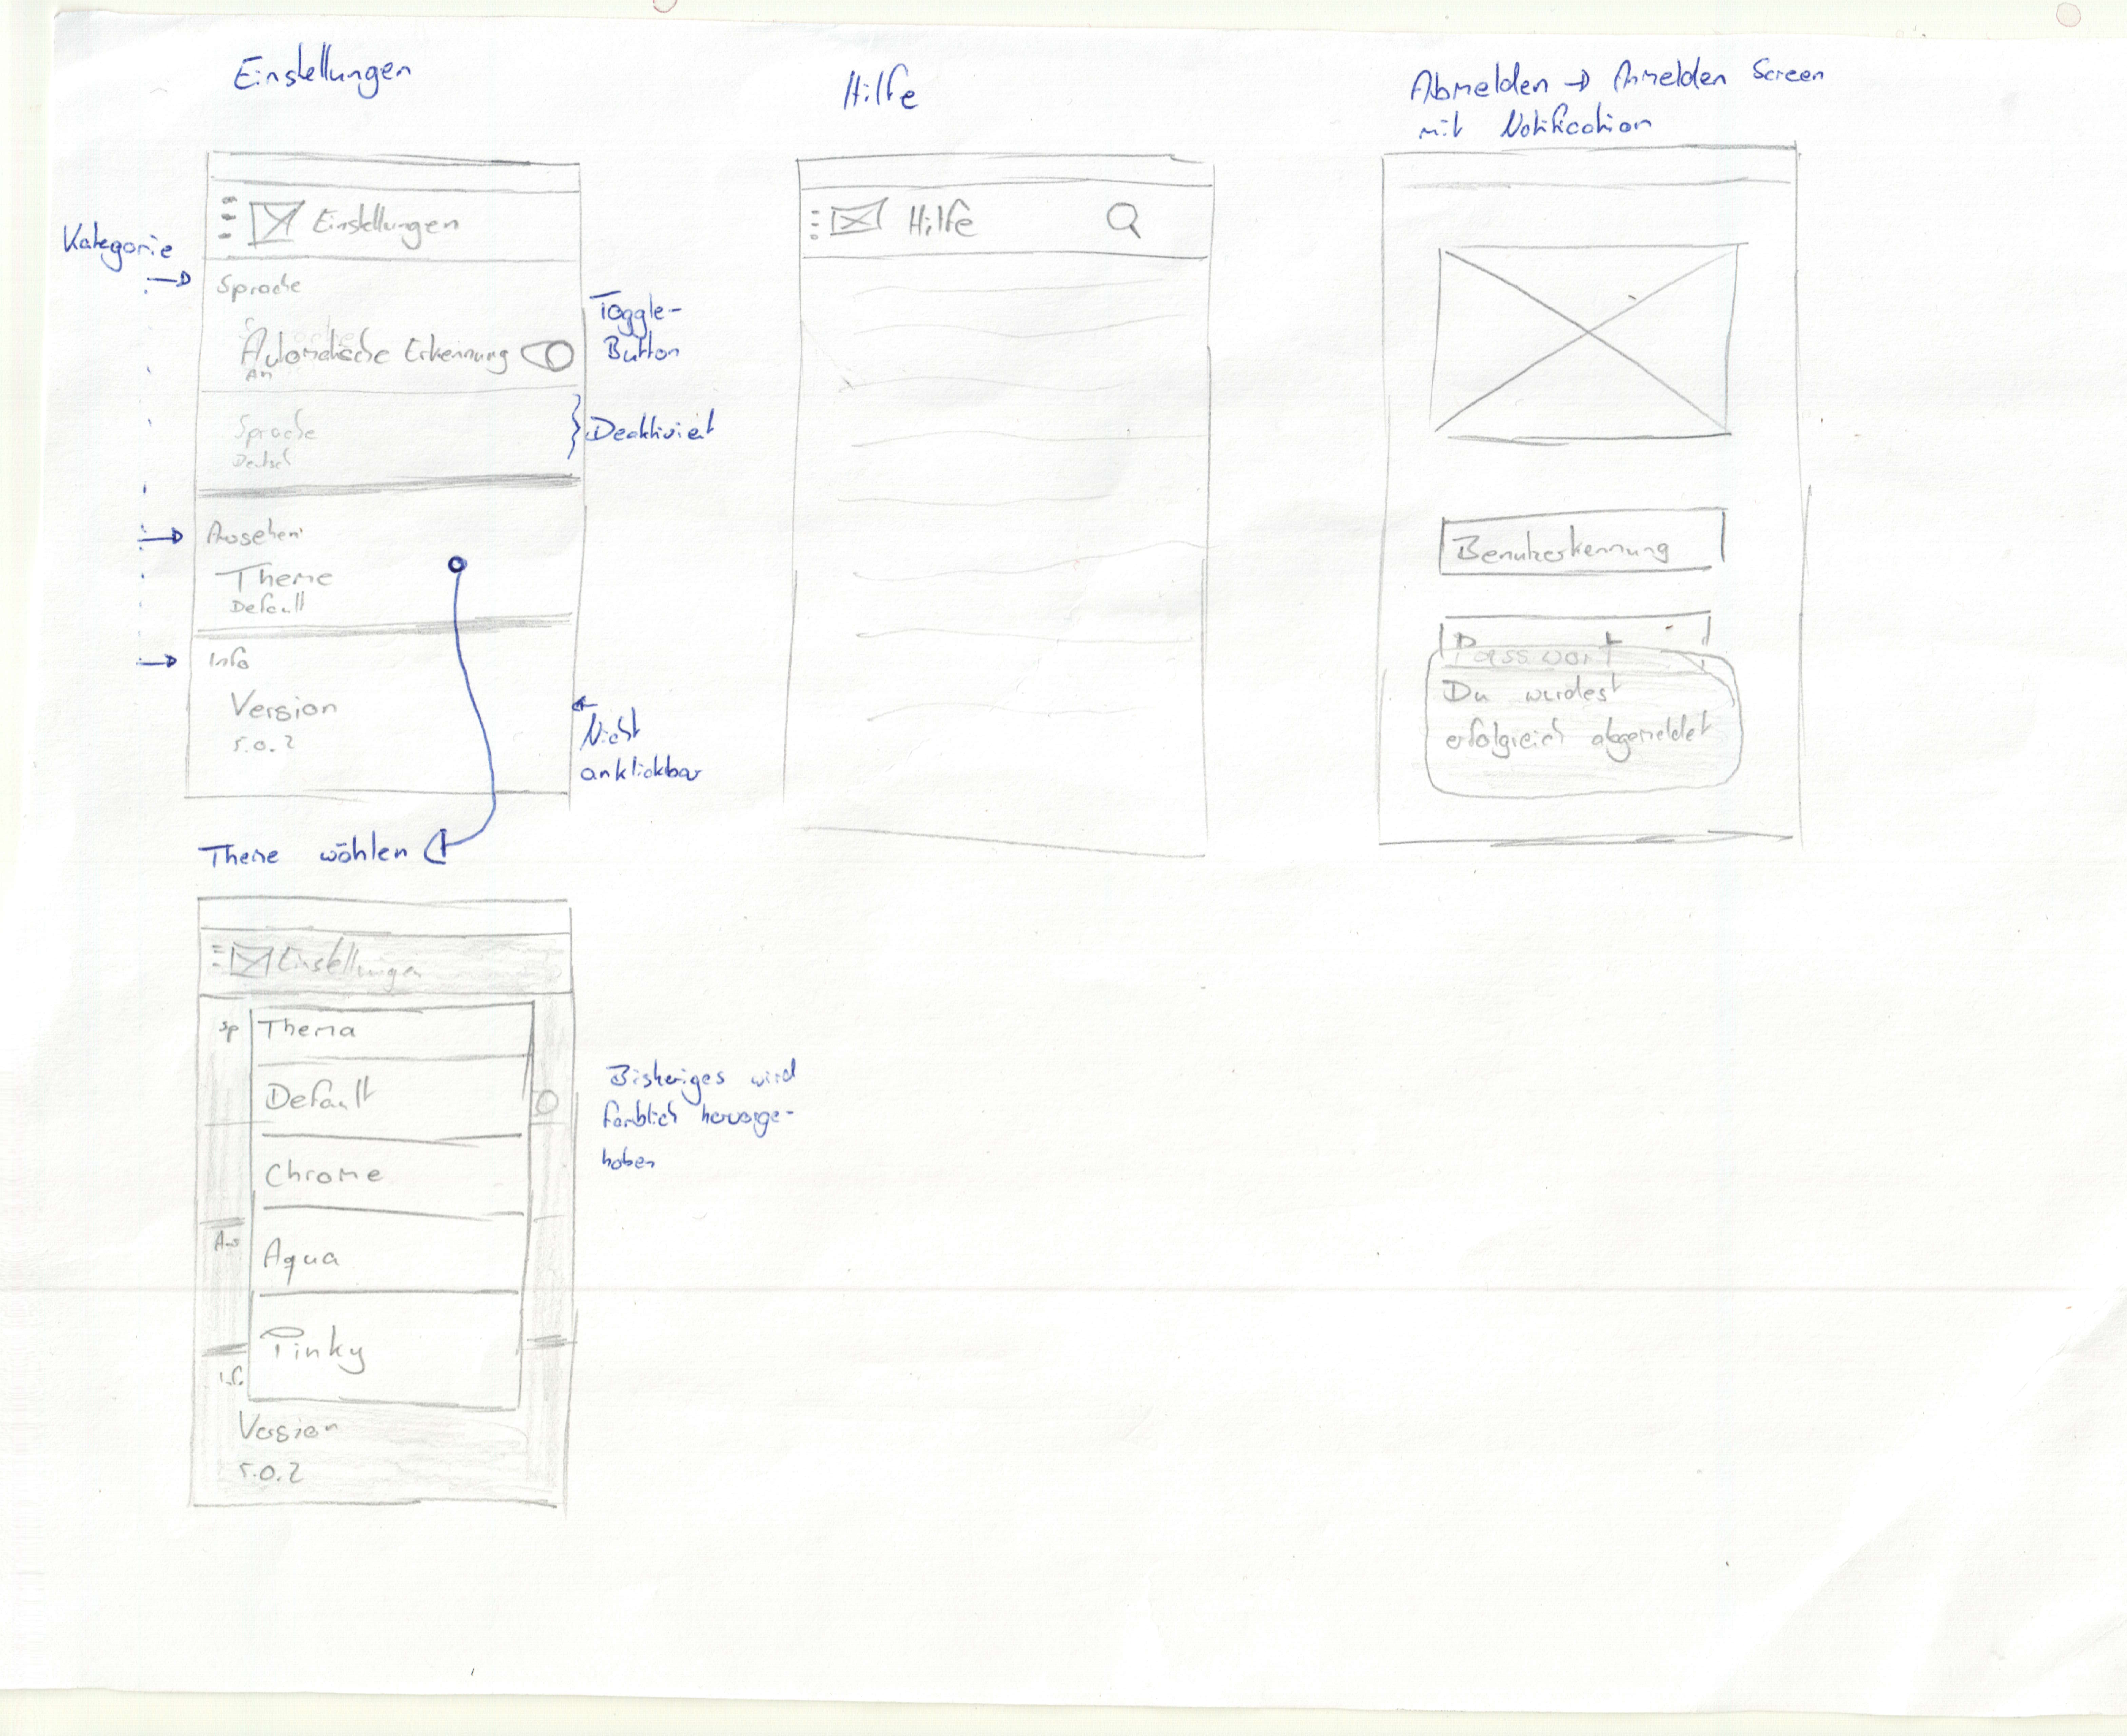
\includegraphics[width=0.99\textwidth]{./images/entwuerfe/toby2}
  \end{center}
  \vspace{-40pt}
\end{wrapfigure}


\clearpage
\begin{wrapfigure}{L}{0.4\textwidth}
  \vspace{-20pt}
  \begin{center}
    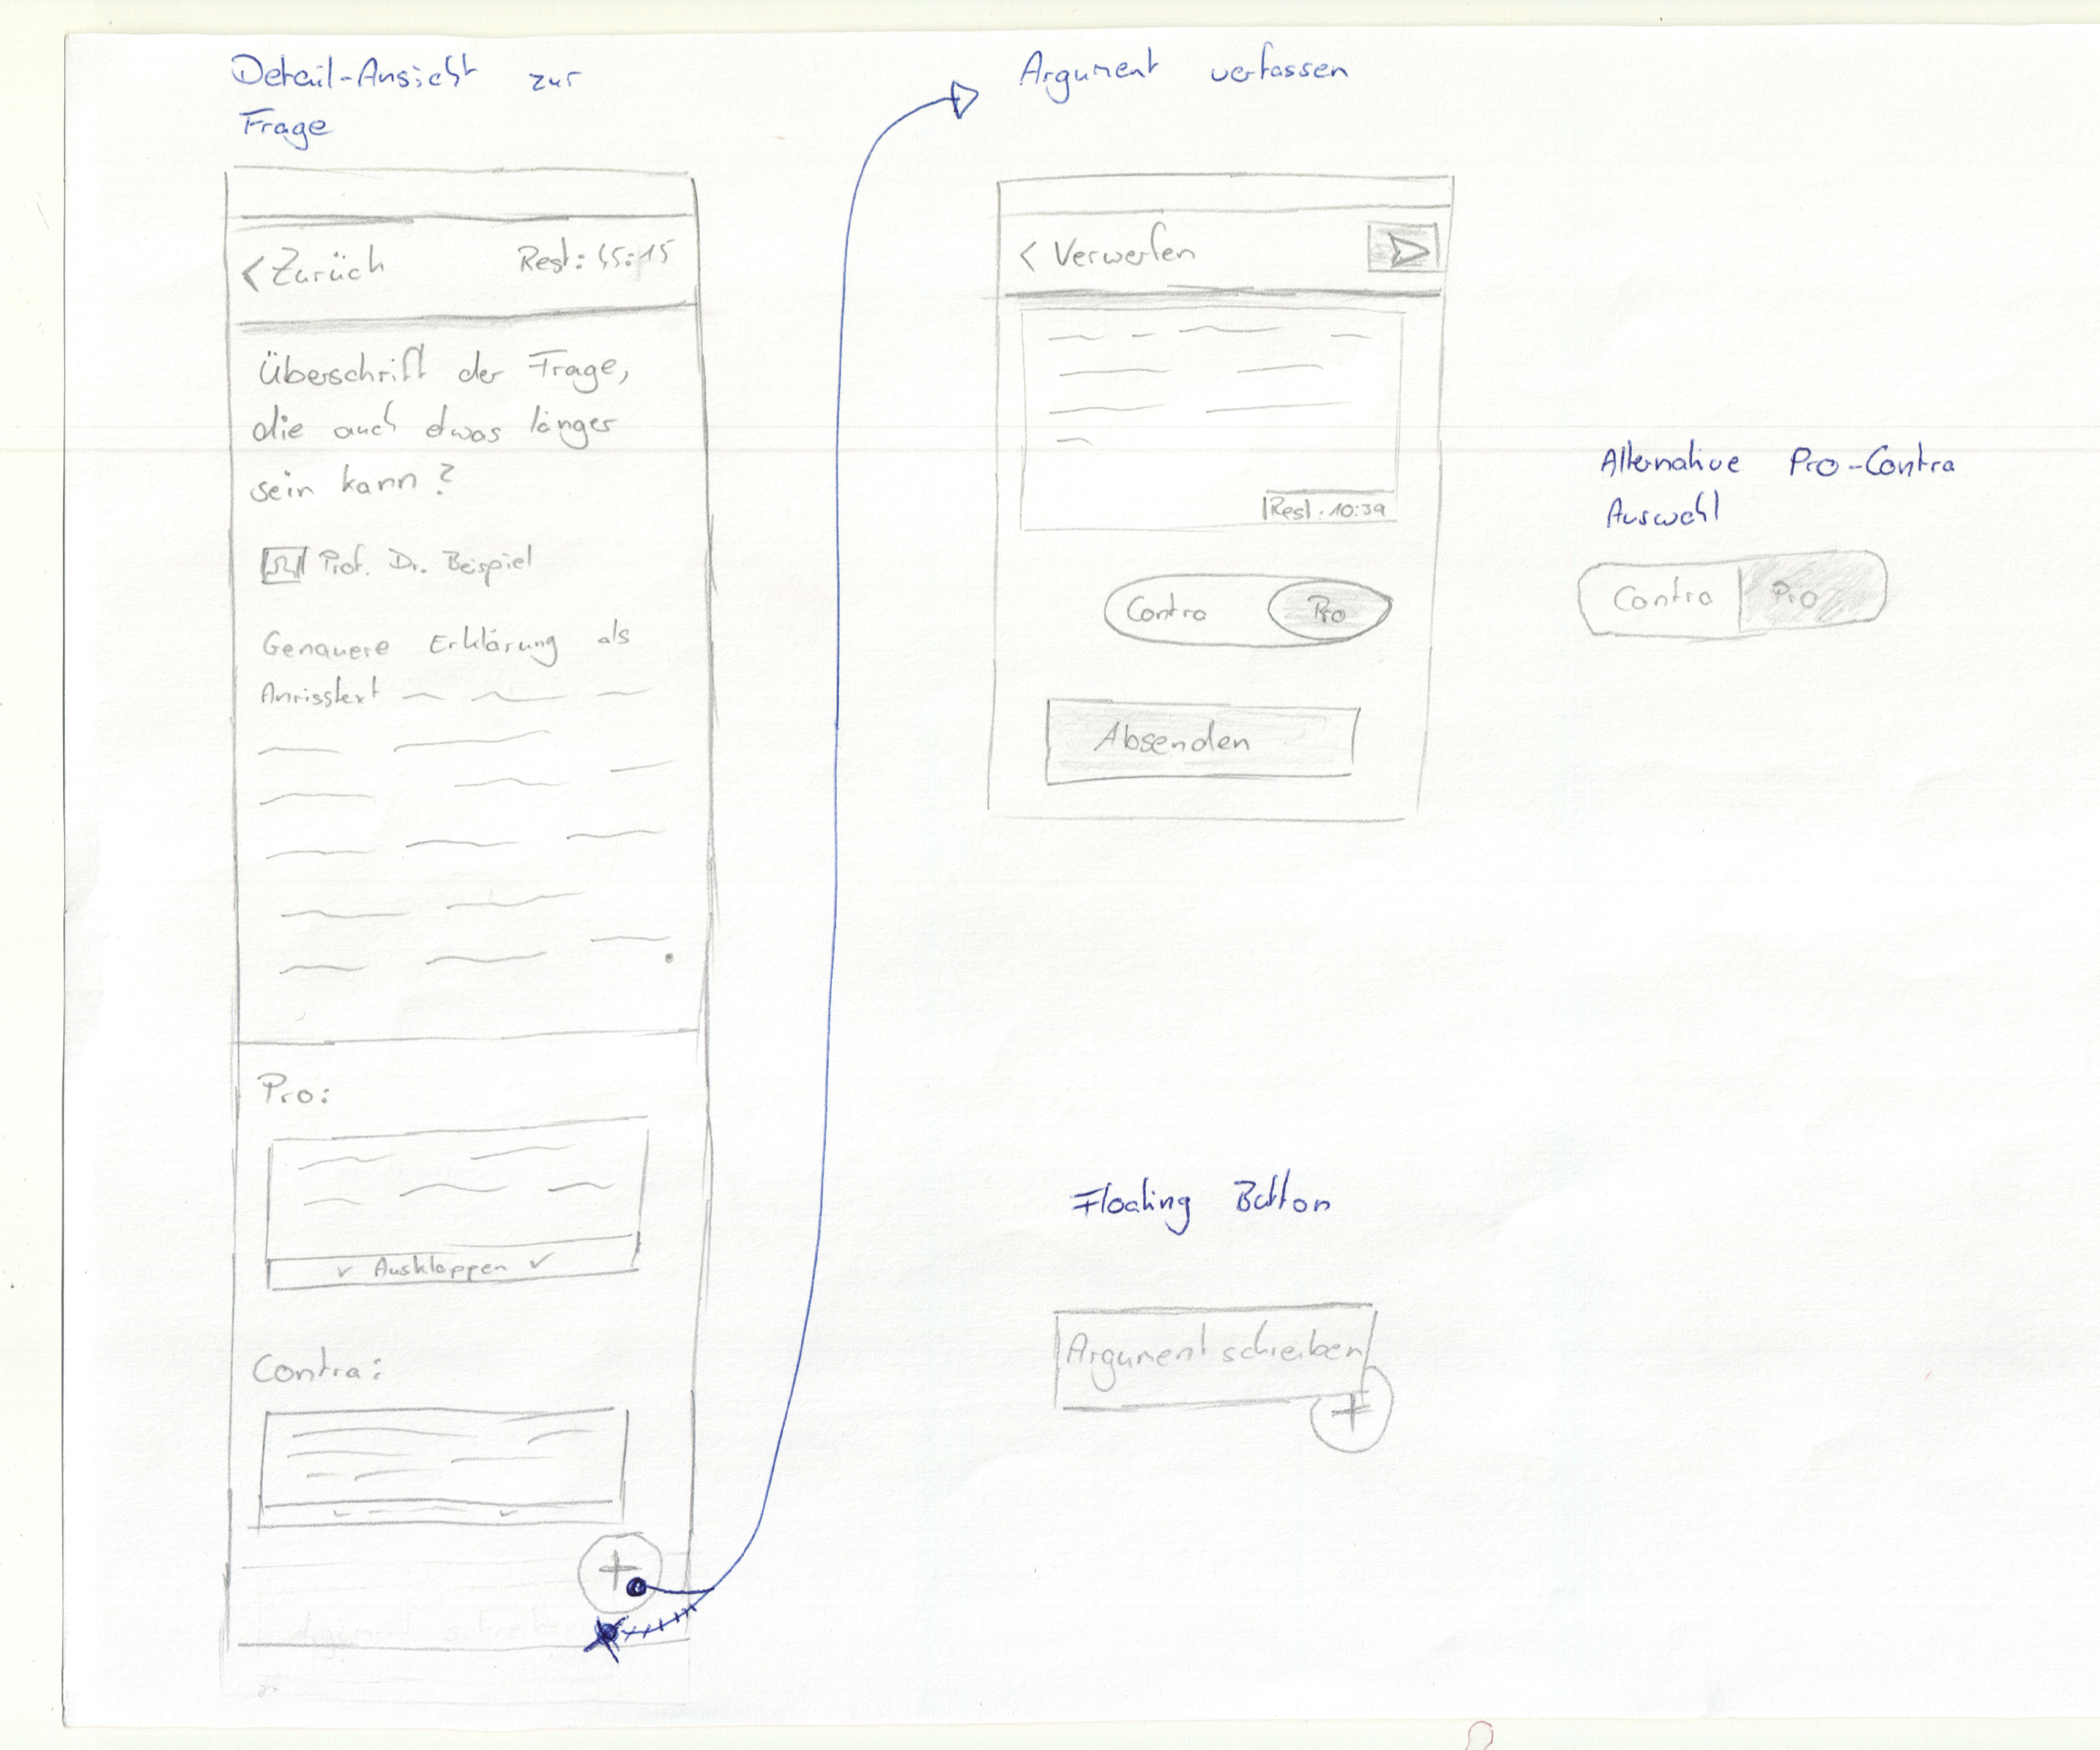
\includegraphics[width=0.99\textwidth]{./images/entwuerfe/toby3}
  \end{center}
  \vspace{-40pt}
\end{wrapfigure}


\clearpage

\section{Best of Storyboard}
\label{sec:bestof}

\subsection{Sprechblasenkommentierung}
\label{sec:sprechblasenkommentierung}

(1 Seite)
Lorem ipsum dolor sit amet, consectetur adipiscing elit. Proin dolor nulla, accumsan non imperdiet convallis, congue nec orci. Nulla id nunc arcu. Fusce a congue metus. Etiam ex nunc, egestas ut urna vitae, commodo ultrices neque. Suspendisse id quam ut nulla sagittis laoreet ut quis nulla. Proin mollis vitae tortor non dignissim. Proin sed nulla eu dolor mattis auctor. Vestibulum eleifend interdum ligula eget pharetra. Integer sollicitudin non arcu non aliquam. Cras placerat ante at pretium vulputate.

Cum sociis natoque penatibus et magnis dis parturient montes, nascetur ridiculus mus. Cras vel augue molestie magna auctor convallis. Nullam tincidunt pharetra orci. Class aptent taciti sociosqu ad litora torquent per conubia nostra, per inceptos himenaeos. Vestibulum congue risus orci, ac accumsan ante pretium et. Vestibulum maximus massa vitae sodales convallis. Integer sed mollis metus, eu porta

\clearpage
\subsection{Objekt-Hierarchie}
\label{sec:objekthierarchie}



\begin{wrapfigure}{L}{0.4\textwidth}
  \vspace{-20pt}
  \begin{center}
    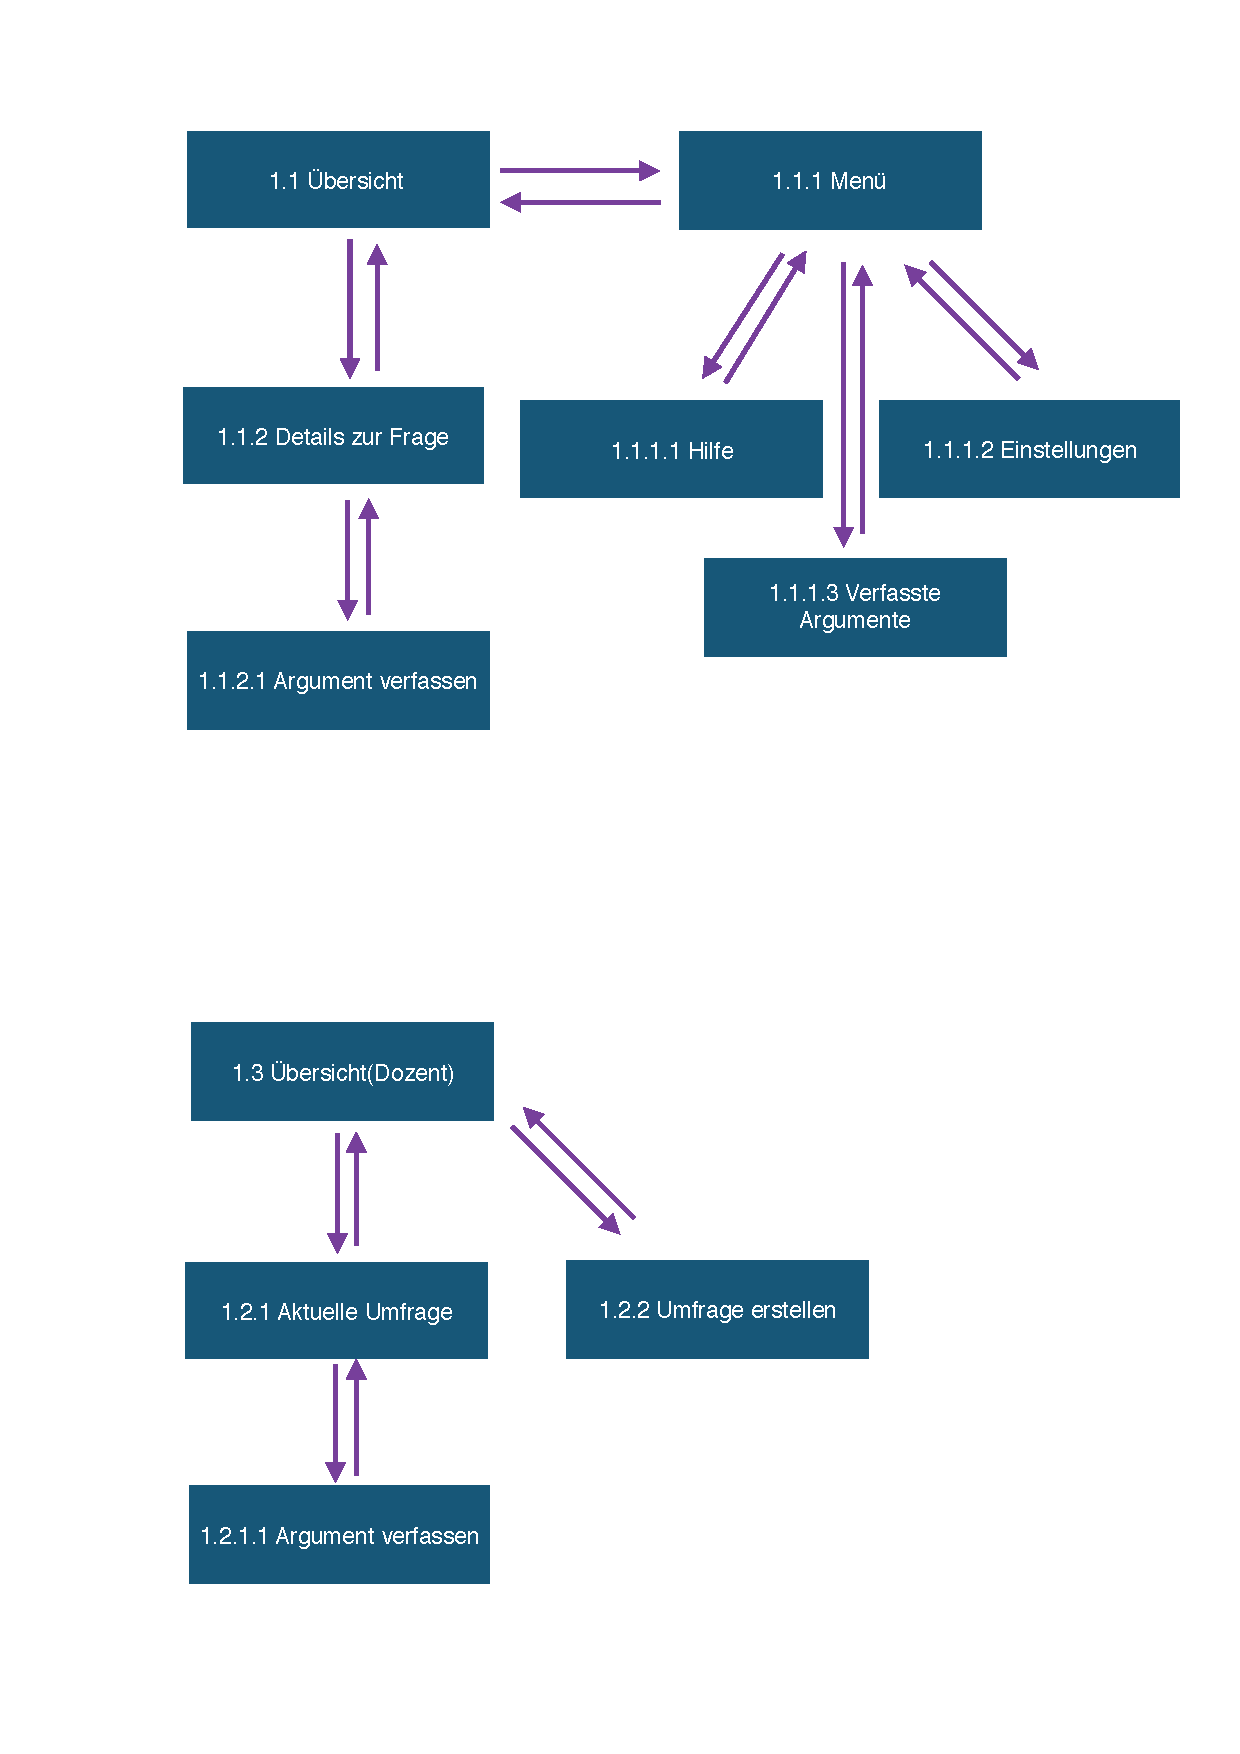
\includegraphics[page=1,width=0.99\textwidth]{./images/objekthierachie}
  \end{center}
  \vspace{-40pt}
\end{wrapfigure}

\clearpage
\subsection{Objekt-Attribut-Aktionen-Tabellen}
\label{sec:objektattribut}

\begin{tabular}{l p{5cm} p{5cm}}
Objekt & Attribute & Aktionen \\
\hline
Übersicht & Aktuelle Fragen, Beendete Fragen & Suchen, Navigieren\\
Menü & Navigationselemente & Navigieren\\
Hilfe & FAQ & Suchen\\
Einstellungen & Sprache, Info, Aussehen & Sprache ändern, Stil ändern, Theme wählen\\
Verfasste Argumente & Abgegebene Argumente & Umfrage aufrufen\\
Detailansicht zur Frage & Überschrift, Beschreibung, Dozent, Pro-Argumente, Kontra-Argumente & Neues Argument erstellen\\
Argument verfassen &Argument, Pro/Kontra & Absenden\\
\end{tabular}

\subsection{Tabelle der Bedienelemente}
\label{sec:bedienelemente}

\bgroup
\def\arraystretch{1.5}
\begin{tabular}{p{4.5cm} | p{1.8cm} p{2cm} p{2.5cm} p{2cm} p{1.8cm} p{2cm}}
Aktion/Attribute & Dedizierter Button & Seitenmenü & Ausklappbares Menü & Toolbar & Android Buttons\\
\hline
Suche &  &  &  & x & x\\
Argument erstellen & x &  &  &  & \\
Argument abschicken & x &  &  & x & \\
Argument verwerfen & x &  &  & x & x\\
Fragen sortieren &  &  & x &  & \\
Fragen nach Aktuellen filtern &  &  & x &  & \\
Einstellungen bearbeiten & x & x &  &  & \\
Hilfe abrufen &  & x &  &  & \\
Fragendetails ausblenden (Zurück zur Übersicht) & x &  &  &  & x\\
\end{tabular}
\egroup

\clearpage

\chapter{Test}
\label{chap:test}

\section{Aufgabenverteilung}

Wir haben die folgende Verteilung beschlossen:\\

\textbf{Testleiter:} Tobias Kerst

Kümmert sich darum, den Test zu erklären und geht die einzelnen Aufgaben mit dem Probanden durch.

\textbf{Unterstützung Testleiter/Interaktionsmanagement:} Maike Rees

Ist für die einzelnen Screens zuständig, dass beim Klicken auf klickbare Elemente die entsprechenden Fenster und Dialoge aufgehen.

\textbf{Protokollant:} Patrick König

Ist für die Dokumentation des Tests zuständig. Hierbei wird der Test an sich und die Nachbesprechung festgehalten.

\section{Testvorbesprechungs-Anleitung}
\label{sec:testvorbesprechung}

Die hier genannten Punkte sind die Anweisungen für den Testleiter, wie er den Probanden auf den Test vorbereiten soll. Der Testleiter probiert diese Punkte in einer lockeren Atmosphäre zu erläutern.

\begin{itemize}
\item Dem Probanden muss klargemacht werden, dass nicht er, sondern nur unsere App getestet wird. Dabei soll uns der Proband helfen.

\item Sage dem Probanden, dass wir versuchen, Fehler an der grafischen Oberfläche zu erkennen.

\item Er soll versuchen, sich diese zu merken, wenn ihm etwas komisch vorkommt oder bestimmte Dinge nicht gefunden werden. Wir sind für jeden gefundenen Fehler an der App dankbar.

\item Erkläre dem Teilnehmer, dass er sich bei dem Test so viel Zeit lassen kann, wie er möchte.

\item Erkläre dem Teilnehmer, dass es vollkommen in Ordnung ist, den Test abzubrechen oder eine kleine Pause einzulegen, wenn er will.

\item Erkläre dem Teilnehmer, dass alle Aufzeichnungen/Daten seiner Umfrage nicht weitergegeben werden und lediglich für die Hochschule gebraucht werden.

\item Sage dem Probanden, dass wir aufschreiben, wie lange er für jede Aufgabe benötigt und, dass wir gegebenenfalls Notizen dazu machen.

\item Der Teilnehmer darf sich danach die Notizen anschauen und sagen, falls ihn etwas stört. 

\item Bitte den Teilnehmer um lautes Denken. Dadurch können bestimmte Fehler an der App, die sonst nicht auffallen, schnell gefunden werden.

\item Hole Dein Handy raus und zeige dem Teilnehmer an Hand einer Standardanwendung, wie das laute Denken funktioniert, um ihm die Angst zu nehmen. 

\item Lege zum Beispiel eine Notiz mit der App Evernote an und spiel an den Einstellungen der App herum. Kommentiere jeden Schritt, den du machst.

\item Sage dem Teilnehmer, dass er jeder Zeit fragen stellen kann, und ihm dann geholfen wird. Er soll sich nicht unter Druck gesetzt fühlen.

\item Nun stelle unser Projekt vor. Zeige dem Probanden kurz eine Übersicht der wichtigen Screens und erkläre Ihm, wofür diese zuständig sind. Er soll sich nicht „ins kalte Wasser geschmissen“ fühlen. Auch hier kann er Fragen stellen.

\item Stelle dem Teilnehmer alle Aufgaben vor, die er gleich durchführen wird

\item Haben Sie noch weitere Fragen?
\end{itemize}

Im Anschluss wird dem Probanden noch das folgende Datenschutzformular vorgelegt.


\begin{wrapfigure}{L}{0.4\textwidth}
  \vspace{-20pt}
  \begin{center}
    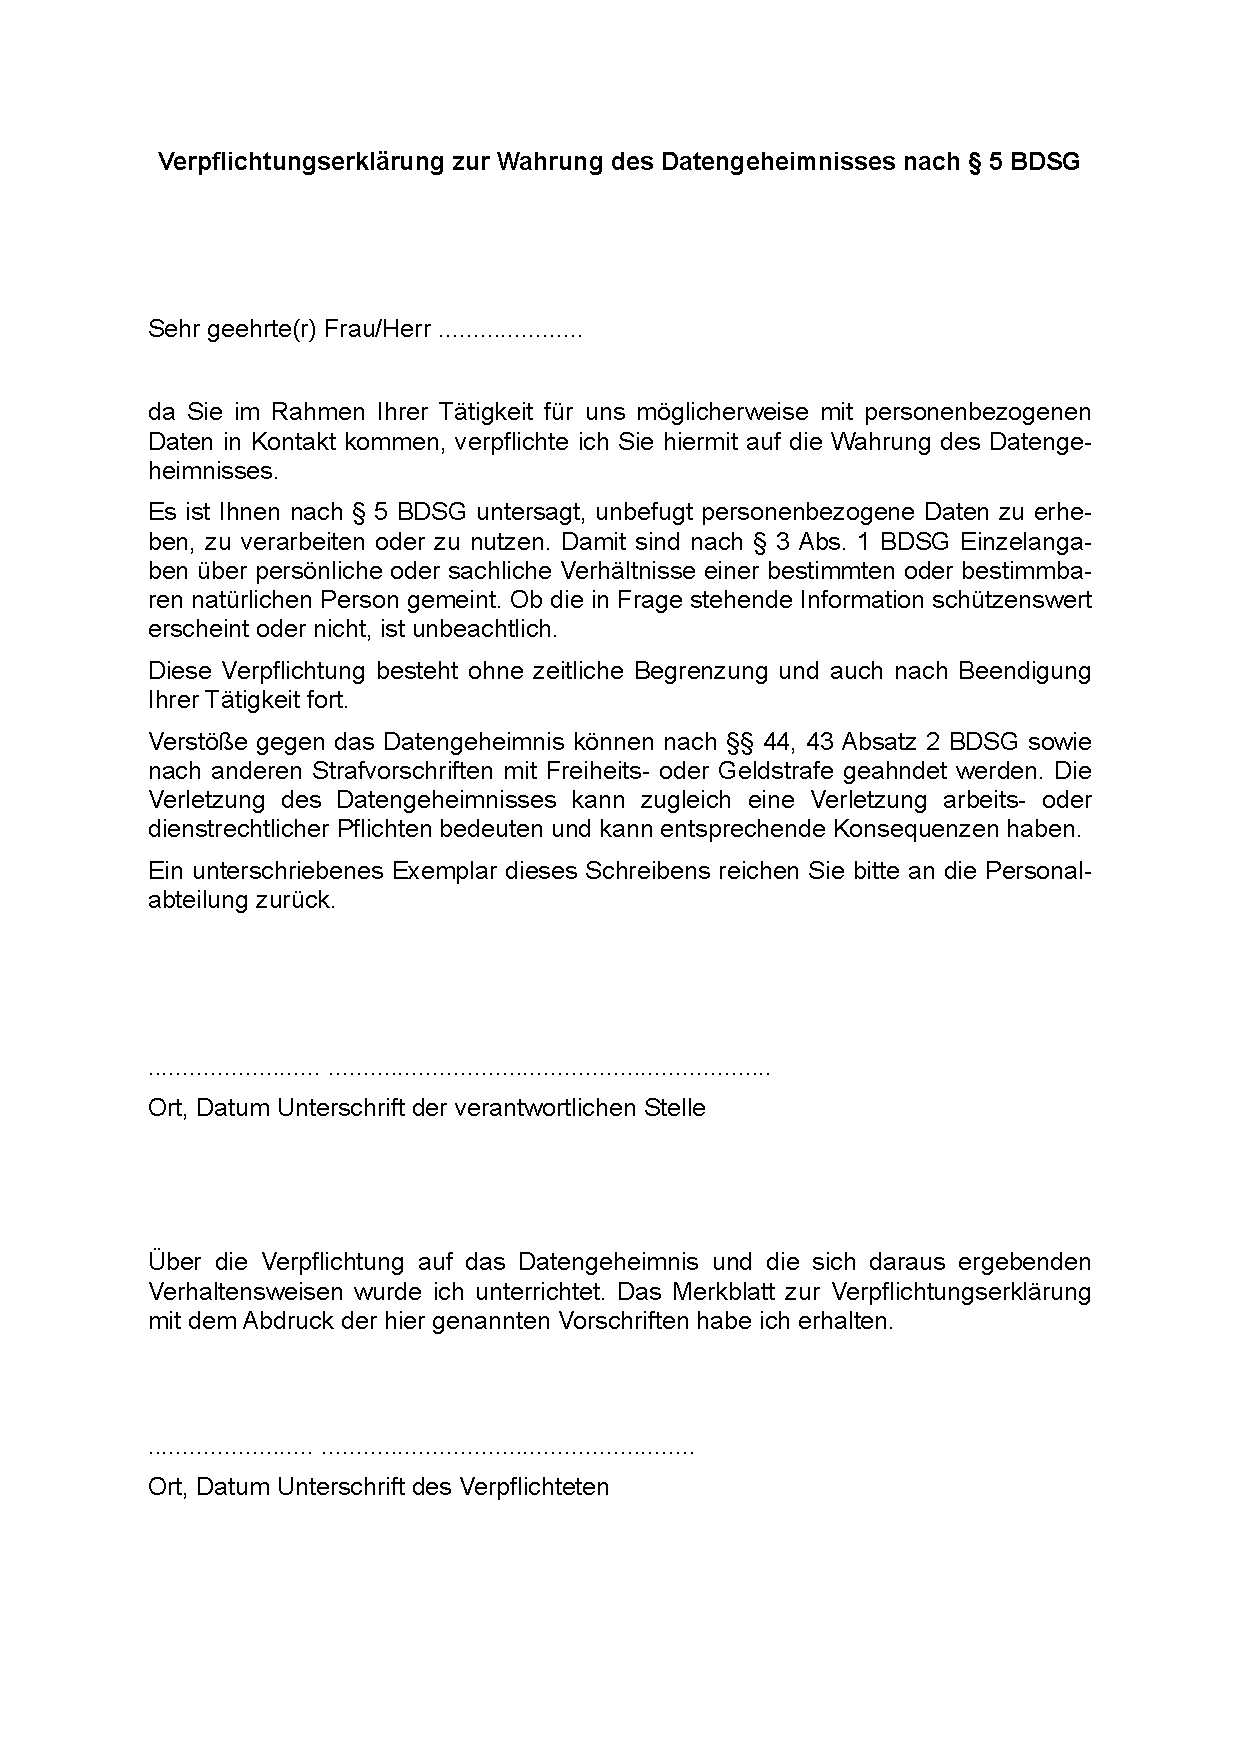
\includegraphics[page=1,width=0.99\textwidth]{./images/datenschutz}
  \end{center}
  \vspace{-40pt}
\end{wrapfigure}

\clearpage

\section{Testfragen}

\begin{wrapfigure}{L}{0.4\textwidth}
  \vspace{-20pt}
  \begin{center}
    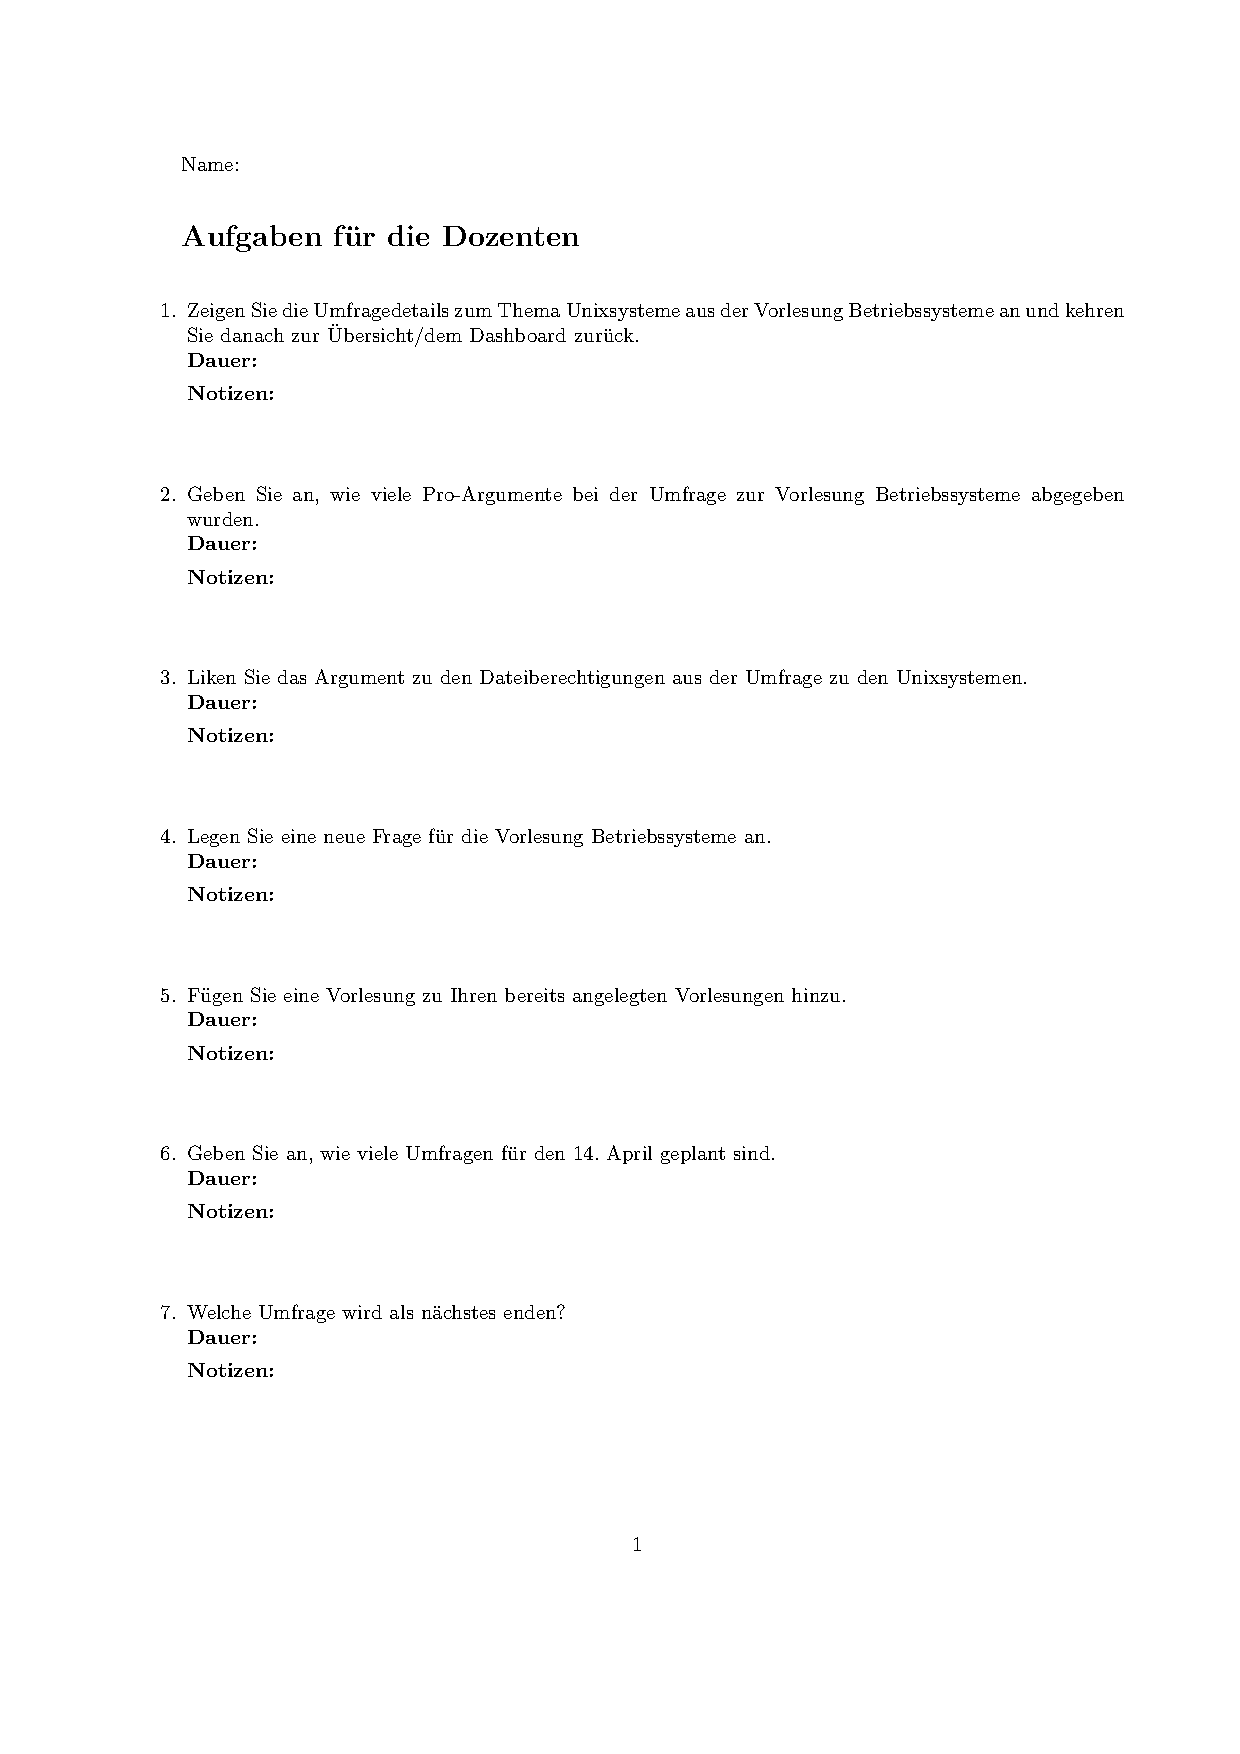
\includegraphics[page=1,width=0.99\textwidth]{./images/probetests}
  \end{center}
  \vspace{-40pt}
\end{wrapfigure}

\begin{wrapfigure}{L}{0.4\textwidth}
  \vspace{-20pt}
  \begin{center}
    \includegraphics[page=2,width=0.99\textwidth]{./images/probetests}
  \end{center}
  \vspace{-40pt}
\end{wrapfigure}

\begin{wrapfigure}{L}{0.4\textwidth}
  \vspace{-20pt}
  \begin{center}
    \includegraphics[page=3,width=0.99\textwidth]{./images/probetests}
  \end{center}
  \vspace{-40pt}
\end{wrapfigure}

\begin{wrapfigure}{L}{0.4\textwidth}
  \vspace{-20pt}
  \begin{center}
    \includegraphics[page=4,width=0.99\textwidth]{./images/probetests}
  \end{center}
  \vspace{-40pt}
\end{wrapfigure}

\clearpage
\section{Nachbefragungs-Formular}
\label{sec:nachbefragung}



\begin{wrapfigure}{L}{0.4\textwidth}
  \vspace{-20pt}
  \begin{center}
    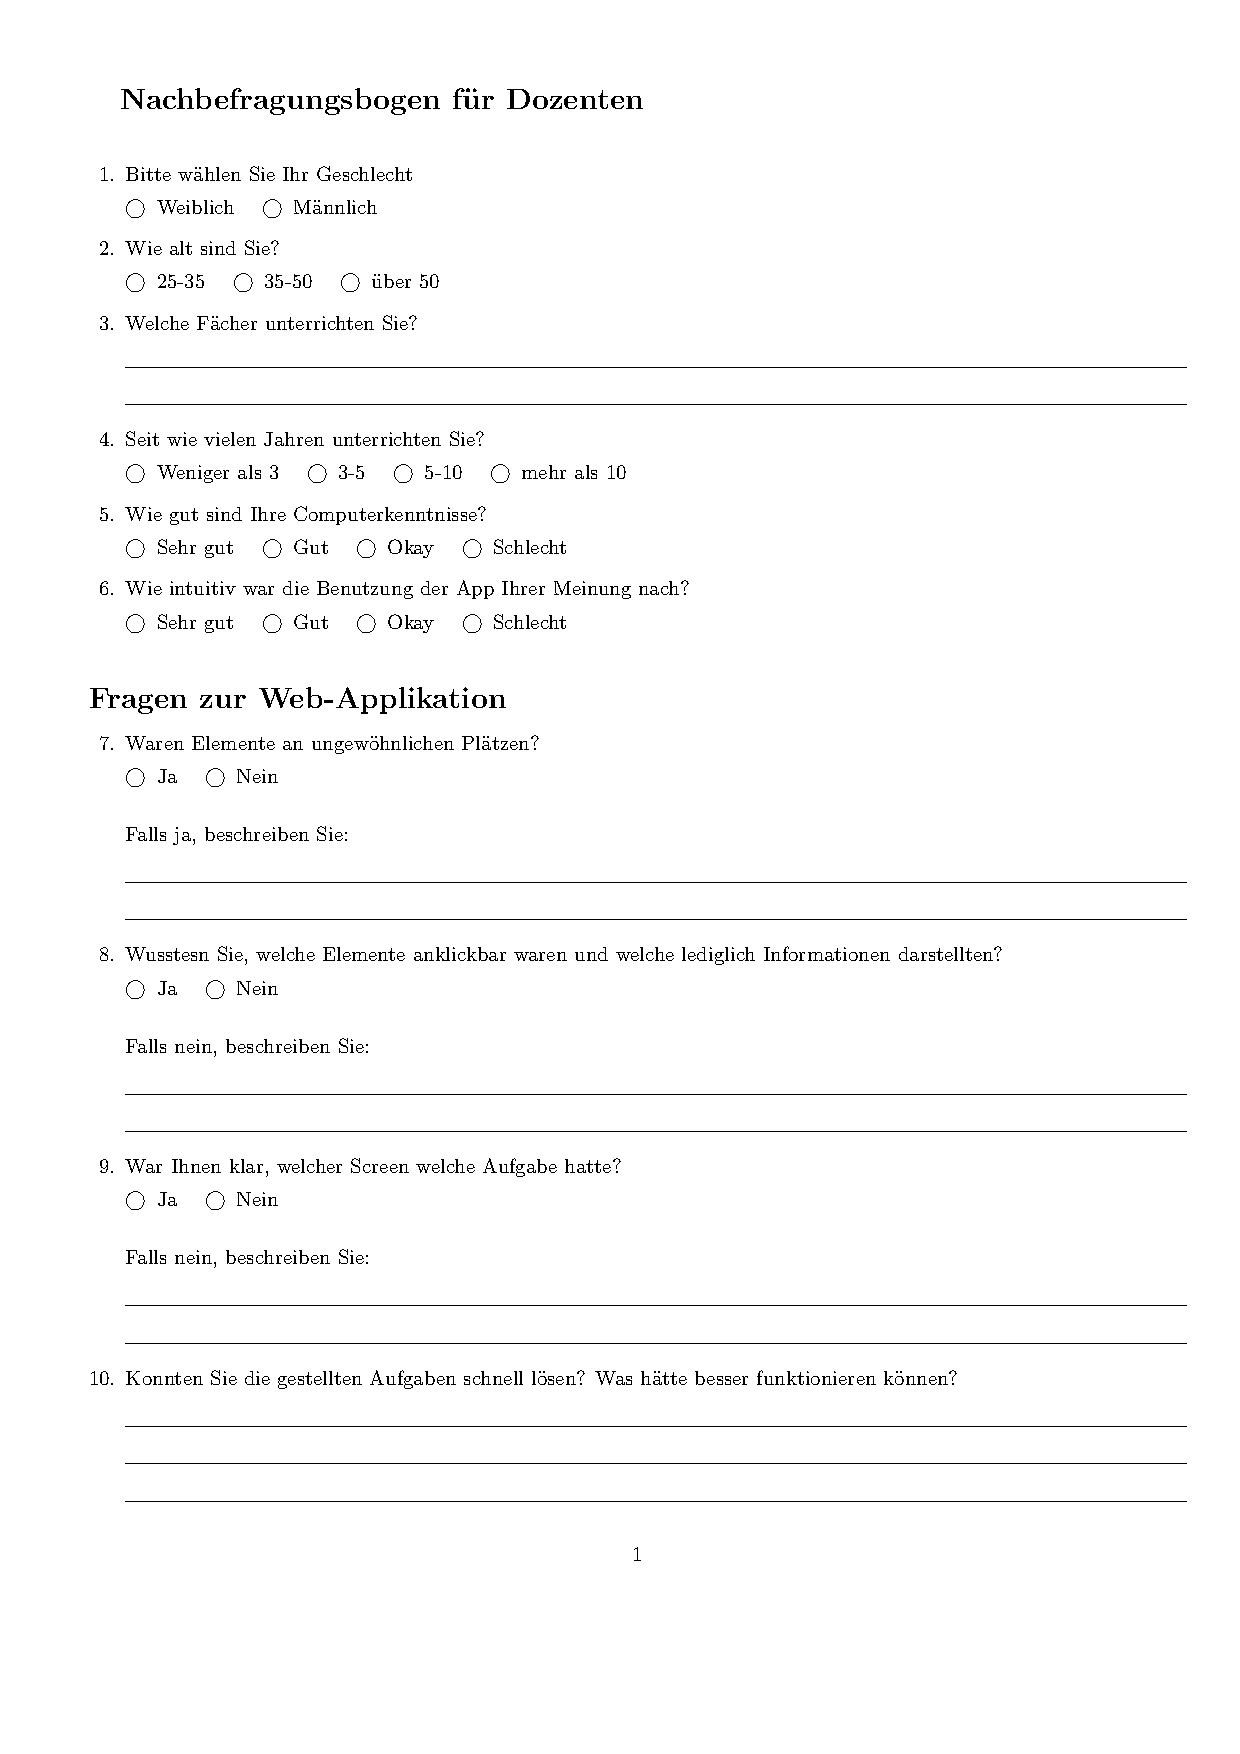
\includegraphics[page=1,width=0.99\textwidth]{./images/dozent}
  \end{center}
  \vspace{-40pt}
\end{wrapfigure}


\begin{wrapfigure}{L}{0.4\textwidth}
  \vspace{-20pt}
  \begin{center}
    \includegraphics[page=2,width=0.99\textwidth]{./images/dozent}
  \end{center}
  \vspace{-40pt}
\end{wrapfigure}


\begin{wrapfigure}{L}{0.4\textwidth}
  \vspace{-20pt}
  \begin{center}
    \includegraphics[page=3,width=0.99\textwidth]{./images/dozent}
  \end{center}
  \vspace{-40pt}
\end{wrapfigure}


\begin{wrapfigure}{L}{0.4\textwidth}
  \vspace{-20pt}
  \begin{center}
    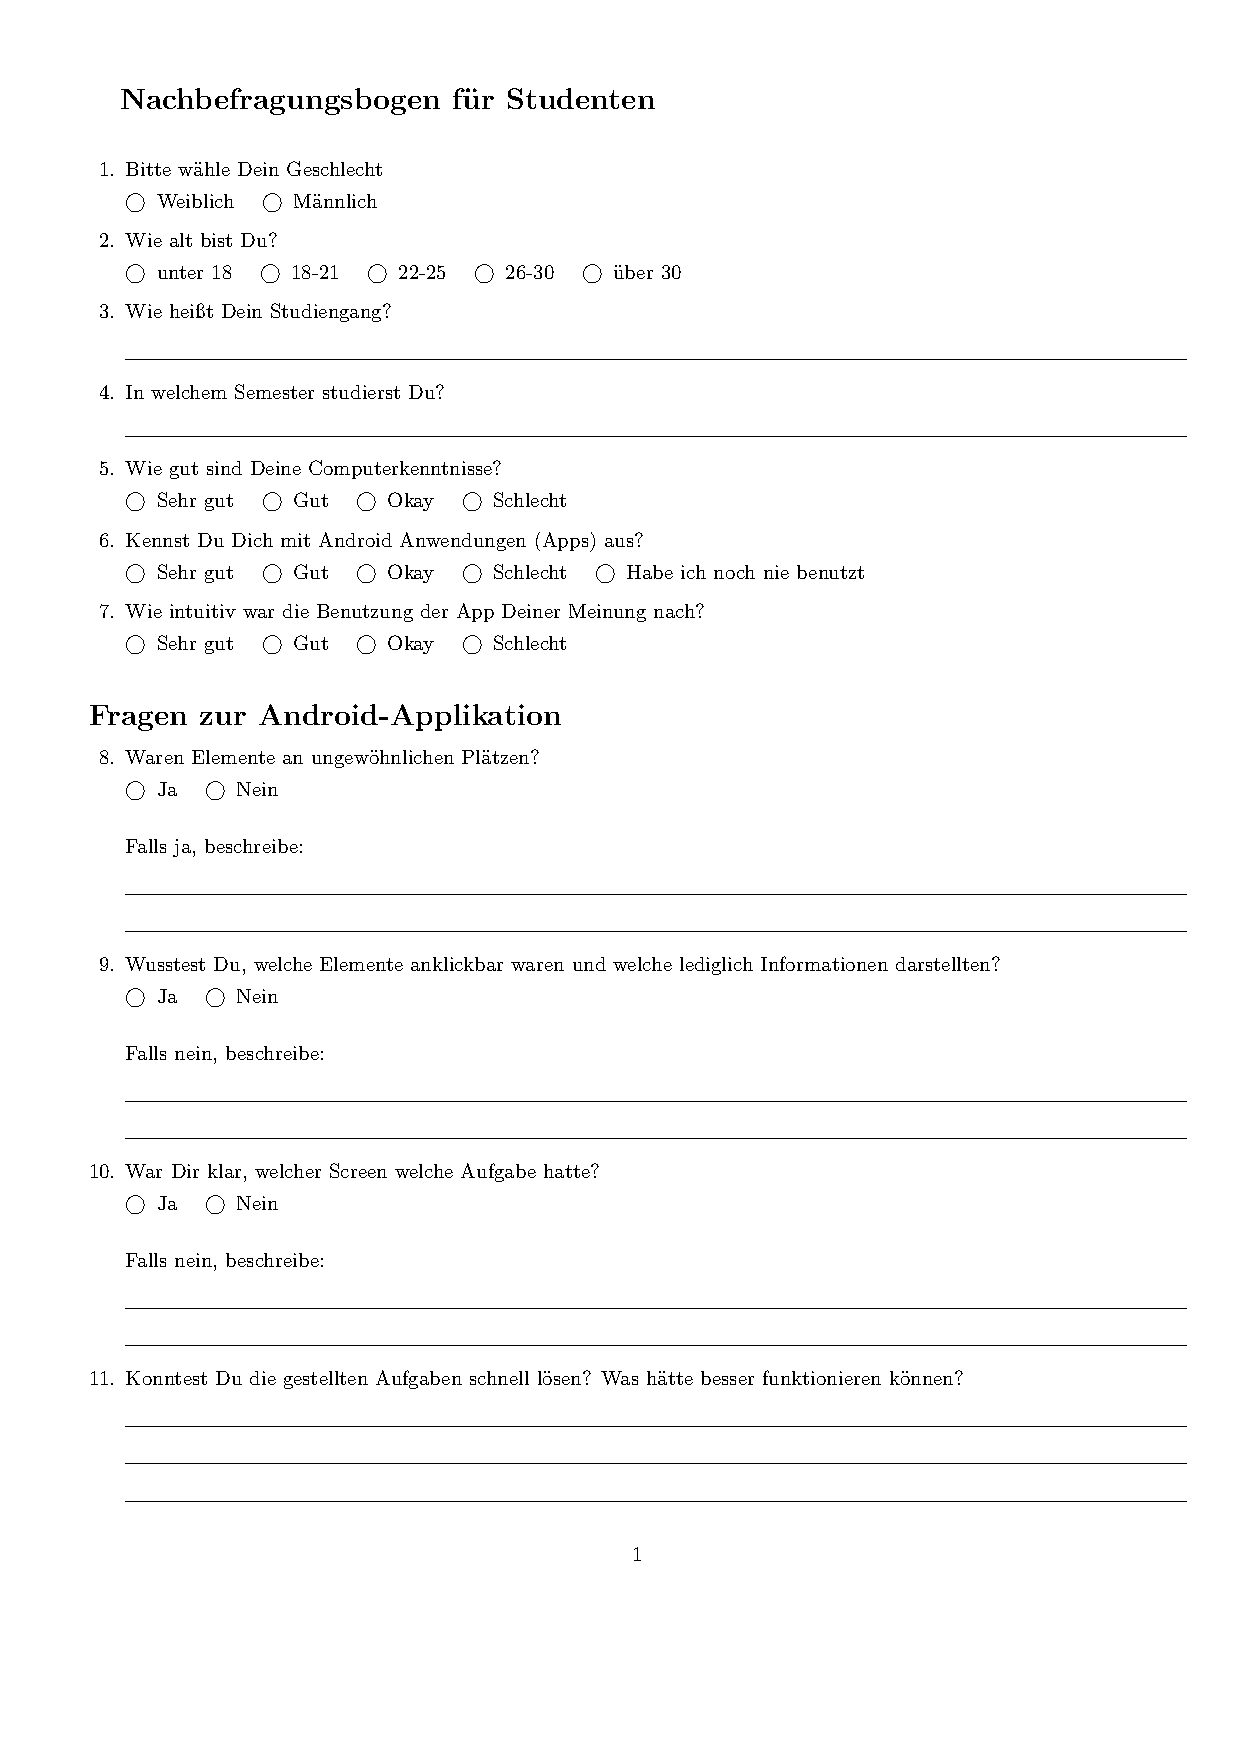
\includegraphics[page=1,width=0.99\textwidth]{./images/student}
  \end{center}
  \vspace{-40pt}
\end{wrapfigure}


\begin{wrapfigure}{L}{0.4\textwidth}
  \vspace{-20pt}
  \begin{center}
    \includegraphics[page=2,width=0.99\textwidth]{./images/student}
  \end{center}
  \vspace{-40pt}
\end{wrapfigure}


\begin{wrapfigure}{L}{0.4\textwidth}
  \vspace{-20pt}
  \begin{center}
    \includegraphics[page=3,width=0.99\textwidth]{./images/student}
  \end{center}
  \vspace{-40pt}
\end{wrapfigure}

\clearpage
\section{Prototypen}
\label{sec:prototypen}

\subsection{Web App}

\begin{wrapfigure}{L}{0.4\textwidth}
  \vspace{-20pt}
  \begin{center}
    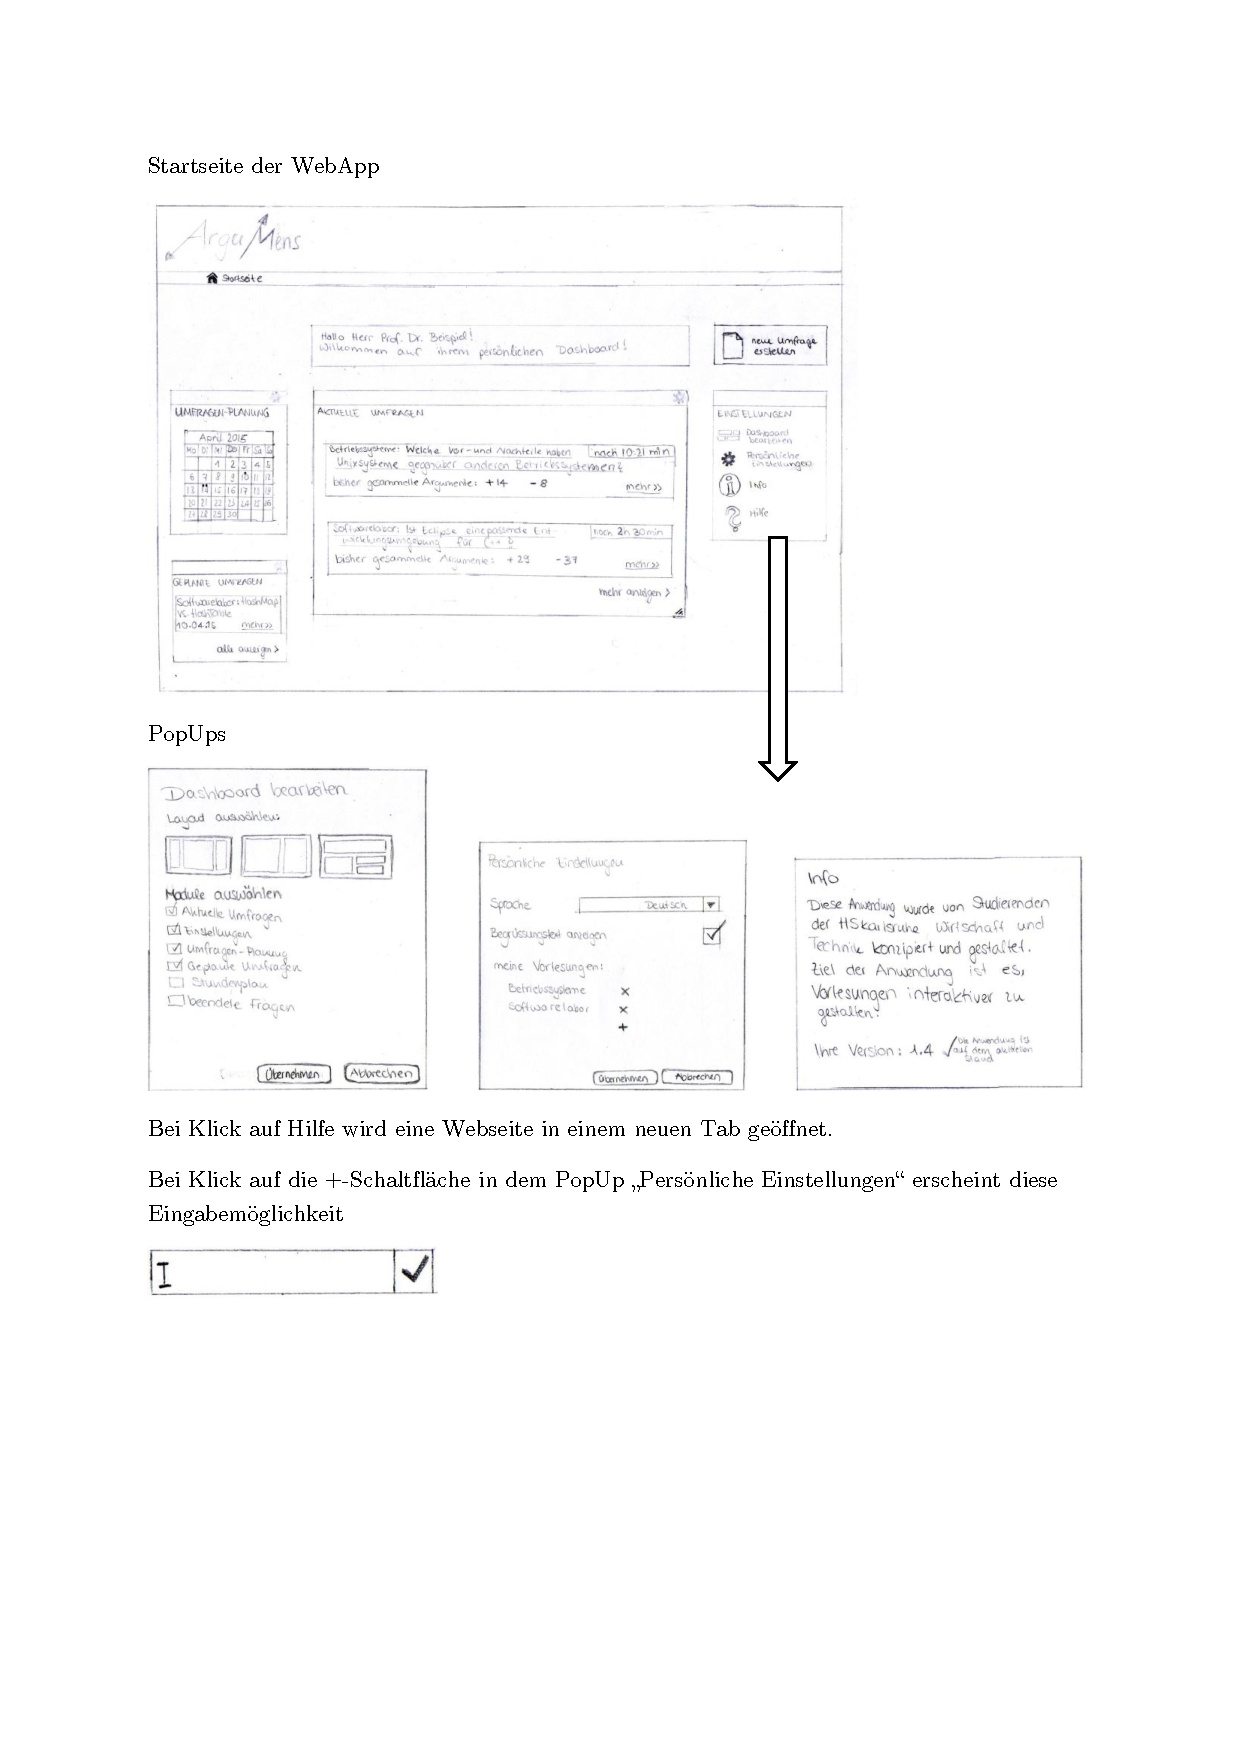
\includegraphics[page=1,width=0.99\textwidth]{./images/prototypWeb}
  \end{center}
  \vspace{-40pt}
\end{wrapfigure}

\begin{wrapfigure}{L}{0.4\textwidth}
  \vspace{-20pt}
  \begin{center}
    \includegraphics[page=2,width=0.99\textwidth]{./images/prototypWeb}
  \end{center}
  \vspace{-40pt}
\end{wrapfigure}

\begin{wrapfigure}{L}{0.4\textwidth}
  \vspace{-20pt}
  \begin{center}
    \includegraphics[page=3,width=0.99\textwidth]{./images/prototypWeb}
  \end{center}
  \vspace{-40pt}
\end{wrapfigure}

\begin{wrapfigure}{L}{0.4\textwidth}
  \vspace{-20pt}
  \begin{center}
    \includegraphics[page=4,width=0.99\textwidth]{./images/prototypWeb}
  \end{center}
  \vspace{-40pt}
\end{wrapfigure}

\begin{wrapfigure}{L}{0.4\textwidth}
  \vspace{-20pt}
  \begin{center}
    \includegraphics[page=5,width=0.99\textwidth]{./images/prototypWeb}
  \end{center}
  \vspace{-40pt}
\end{wrapfigure}

\subsection{Android App}


\begin{wrapfigure}{L}{0.4\textwidth}
  \vspace{-20pt}
  \begin{center}
    \includegraphics[page=1,width=0.99\textwidth]{./images/prototypApp}
  \end{center}
  \vspace{-40pt}
\end{wrapfigure}


\begin{wrapfigure}{L}{0.4\textwidth}
  \vspace{-20pt}
  \begin{center}
    \includegraphics[page=2,width=0.99\textwidth]{./images/prototypApp}
  \end{center}
  \vspace{-40pt}
\end{wrapfigure}


\begin{wrapfigure}{L}{0.4\textwidth}
  \vspace{-20pt}
  \begin{center}
    \includegraphics[page=3,width=0.99\textwidth]{./images/prototypApp}
  \end{center}
  \vspace{-40pt}
\end{wrapfigure}


\begin{wrapfigure}{L}{0.4\textwidth}
  \vspace{-20pt}
  \begin{center}
    \includegraphics[page=4,width=0.99\textwidth]{./images/prototypApp}
  \end{center}
  \vspace{-40pt}
\end{wrapfigure}


\begin{wrapfigure}{L}{0.4\textwidth}
  \vspace{-20pt}
  \begin{center}
    \includegraphics[page=5,width=0.99\textwidth]{./images/prototypApp}
  \end{center}
  \vspace{-40pt}
\end{wrapfigure}


\clearpage
\section{Vorherige Probetests}
\label{sec:probetests}

(2 Seiten)

Lorem ipsum dolor sit amet, consectetur adipiscing elit. Proin dolor nulla, accumsan non imperdiet convallis, congue nec orci. Nulla id nunc arcu. Fusce a congue metus. Etiam ex nunc, egestas ut urna vitae, commodo ultrices neque. Suspendisse id quam ut nulla sagittis laoreet ut quis nulla. Proin mollis vitae tortor non dignissim. Proin sed nulla eu dolor mattis auctor. Vestibulum eleifend interdum ligula eget pharetra. Integer sollicitudin non arcu non aliquam. Cras placerat ante at pretium vulputate.

Cum sociis natoque penatibus et magnis dis parturient montes, nascetur ridiculus mus. Cras vel augue molestie magna auctor convallis. Nullam tincidunt pharetra orci. Class aptent taciti sociosqu ad litora torquent per conubia nostra, per inceptos himenaeos. Vestibulum congue risus orci, ac accumsan ante pretium et. Vestibulum maximus massa vitae sodales convallis. Integer sed mollis metus, eu porta

\section{Testbericht}
\label{sec:testbericht}

\subsection{Im Test erkannte Probleme}
\label{sec:foundproblemes}

Durch den Test der Android-App sind einige Schwächen unseres Prototypen aufgefallen. Besonders hervorzuheben ist hier die Struktur der App.

Beispielsweise ist bereits zu Beginn aufgefallen, dass dem Probanden nicht klar war, was auf dem Homescreen dargestellt wird und was nicht. Wir hatten uns dazu entschlossen, auch bereits abgelaufene Umfragen unter den aktuellen Umfragen aufzulisten, was offensichtlich zur Verwirrung geführt hat. Somit war es für den Probanden nicht klar, dass wir einen separaten Screen für die von ihm abgegebenen Argumente haben, was quasi einem Archiv entspricht.

Als nächstes stellten wir fest, dass der Proband Schwierigkeiten damit hatte die globalen Einstellungen von den Ansichtseinstellungen des Homescreens zu unterscheiden. Gemeint sind hier die Einstellungen zum Ausblenden von bereits abgelaufenen Umfragen und der Sortierung aller Umfragen. Der Button, der dieses Menü aufruft, wurde erst sehr spät gefunden.

Es wurde angemerkt, dass die App in gewissen teilen sehr intuitiv, wie beim Verfassen der Argumente oder dem Aktualisieren der Umfragen, aber auch teilweise aufgrund der verbesserungswürdigen Struktur nicht absolut intuitiv war.
Außerdem muss die Suche verbessert werden um auch abgegebene Argumente zu finden.

Zuletzt viel auf, dass (vor allem auf dem Homescreen) nicht immer klar war, was anklickbar ist und was nicht. Dies wurde offenkundig, als der Proband auf einzelne Teile einer Umfragekachel klickte und eine gewisse Ausgabe erwartete. Dabei sind die Kacheln als Einheit zu sehen.

\subsection{Abgeleitete Verbesserungsvorschläge}
\label{sec:verbesserungsvorschlaege}

Man kann aus denen im Test festgestellten Problemen einige Verbesserungsvorschläge ableiten. Zum Einen sollte man definitiv die Struktur der App überdenken. Der Homescreen sollte die bereits abgelaufenen Umfragen nicht weiter anzeigen, sondern in einen gesonderten Screen auslagern, den man als Archiv bezeichnen kann. Hierbei ist dann noch wichtig, dass eine Differenzierung der bereits abgelaufenen Umfragen und der von dem Benutzer abgegebenen Argumente zu allen (auch abgelaufenen) Umfragen notwendig ist. Wie man diese Teile am besten trennt, müsste durch weitere Tests herausgefunden werden. Dadurch, dass diese Funktionalität jedoch vermutlich nur selten genutzt wird und daher keine wichtige Funktion ist, sollte man diese Screens in das Slide-In Menü integrieren, da dieses Menü primär genutzt wird, wenn man erweiterte Funktionen benötigt.

Außerdem sollte man die Sortierung der Umfragen in die bereits existierenden Einstellungen auslagern, da die App somit noch simpler wird.

Zuletzt muss man, wie oben angemerkt, die Suche verbessern und verfeinern und die anklickbaren Elemente grafisch verbessern.

\subsection{Kritik und Bewertung des Tests}
\label{sec:kritik}

Beim Test unseres Prototypen sind uns einige Dinge aufgefallen, die primär konzeptioneller Natur waren. Es hat bereits damit angefangen, dass wir durch technische Probleme nicht alle Dokumente ausdrucken konnten und somit dann auch zu spät zu dem verabredeten Test gekommen sind. Daraus entstand dann eine entsprechend gestresste Situation, die man durch bessere Planung hätte umgehen können. 
Nachdem wir dann alles für den Test gerichtet hatten fiel relativ schnell auf, dass wir unsere App zu ausführlich testen wollten und dass wir uns nicht auf spezielle Fälle fokussierten. Wir wollten sowohl die Webapplikation, als auch die Android App testen und hatten dafür sehr viele Testfälle vorbereitet, was auch dem Testleiter bewusst war. Daraus resultierte, dass die Testvorbesprechung viel zu kurz kam und eventuelle Fragen eventuell nicht geklärt wurden.
Beim eigentlichen Test haben wir dann festgestellt, dass die eigentlichen Funktionen erst viel zu spät dran kamen, so hatten wir als ersten Fall gefragt, wie man Einstellungen ändert und das Archiv findet und daraus Informationen ableitet. Es wäre an dieser Stelle wesentlich sinnvoller gewesen, wenn man zuerst die Abfrage von Informationen zu den existierenden Umfragen gefordert hätte, da sich der Proband dann auch schneller an den strukturellen Aufbau der App hätte gewöhnen können und somit die Aufgaben schneller hätte lösen können. Durch unsere Fragen verwirrten wir den Probanden jedoch massiv, was während dem Test alles andere als förderlich war.

Wie bereits angesprochen, haben wir die Testdauer unterschätzt, so kam es dazu, dass wir Testaufgaben überspringen mussten und der Prototyp für die Webapp überhaupt nicht getestet wurde. In Zukunft ist eine bessere Abschätzung des Verlaufs von essenzieller Bedeutung.

Es fiel zudem auf, dass der Testleiter während des Tests die Aktionen des Probanden in einigen Fällen durch seine Aussagen bewertete. Dies sollte, wie in der Anfangsbesprechung auch gefordert, vermieden werden.

Auch wenn nicht alles absolut perfekt funktioniert hat, kann man festhalten, dass wir durch die gemachten Fehler viel gelernt haben, was man in Zukunft vermeiden kann.

\clearpage


\end{document}
